\section{Problem and numerical framework}

The study asks whether a strong RBF--FD-specific preconditioner leaves a reproducible inverse action that learning can exploit. A direct model may learn the full missing action without assuming low dimension. A subspace model becomes meaningful only after a compact, stable, solver-relevant difficult space has been demonstrated. Proper orthogonal decomposition (POD) therefore serves as a diagnostic and classical reference. This framework defines the alternatives tested throughout the report.

The complete computational framework is summarized here before the empirical development.  Consider
\begin{equation}
 -\nabla\!\cdot\!\bigl(K(x)\nabla u(x)\bigr)=f(x),\qquad x\in\Omega=[0,1]^2,
 \qquad u=g\ \text{on }\partial\Omega ,
 \label{eq:pde}
\end{equation}
where $K=I$ gives Poisson, $K=a(x)I$ gives scalar diffusion, and $K$ may be a symmetric positive-definite tensor.  Manufactured sine-series solutions provide analytic forcing and boundary data.  Thus discretization error and linear-solver residual are measured separately.

\subsection{Local RBF--FD operator}

The established experiments use quasi-uniform tensor-product nodes with fixed boundary nodes and reproducible interior jitter.  At each interior point $x_i$, a $k$-d tree returns the $s$ nearest nodes $S_i$.  The stencil is translated by $x_i$ and divided by its farthest-node radius $\rho_i$.  With the polyharmonic spline
\begin{equation}
 \phi(r)=r^3
 \label{eq:phs}
\end{equation}
and all monomials of total degree at most two,
$p=(1,x,y,x^2,xy,y^2)$, the local weights solve
\begin{equation}
 \begin{bmatrix}\Phi_i&P_i\\P_i\trans&0\end{bmatrix}
 \begin{bmatrix}w_i\\\lambda_i\end{bmatrix}
 =
 \begin{bmatrix}\mathcal L_i\phi(\norm{\cdot-x_j})|_{x_i}\\
                 \mathcal L_i p|_{x_i}\end{bmatrix}.
 \label{eq:weights}
\end{equation}
Here $(\Phi_i)_{jk}=\phi(\norm{\widehat x_j-\widehat x_k})$ and $P_i$ evaluates the scaled monomials.  First derivatives are rescaled by $\rho_i^{-1}$ and second derivatives by $\rho_i^{-2}$.  No regularization or silent least-squares fallback is used.  A failed local augmented solve is recorded as an invalid node set.

For constant $K$, $\mathcal L u=-K_{11}u_{xx}-2K_{12}u_{xy}-K_{22}u_{yy}$.  For a spatial tensor, the implementation includes the product-rule drift exactly,
\begin{equation}
 \mathcal L u=-K:\nabla^2u-(\nabla\!\cdot K)\cdot\nabla u.
 \label{eq:variableoperator}
\end{equation}
Each interior row inserts $w_i$ only at stencil columns.  A boundary row is the corresponding identity row and its right-hand side is the manufactured Dirichlet value.  The result is the sparse, generally nonsymmetric system $Au=b$.  
\subsection{Classical and complementary inverse actions}

The principal baseline is SuperLU threshold ILU with drop tolerance $10^{-3}$, fill factor 5, COLAMD ordering, and zero diagonal-pivot threshold.  It defines a fixed linear inverse action $M^{-1}$ \citep{saad1994ilut}.  An early RBF--FD-specific control assembles a cheaper matrix $B_s$ on the same nodes with a smaller stencil and applies $\ilu(B_s)^{-1}$ \citep{koch2025smaller}.  Later experiments retain the stronger $\ilu(A)$ baseline.

For any residual or Arnoldi vector $r$, the exact missing inverse action is
\begin{equation}
 d(r)=A^{-1}r-M^{-1}r.
 \label{eq:missing}
\end{equation}
The term $A^{-1}r$ is always obtained from an accurate solve, never by forming an inverse.  With training snapshots $D=[d^{(1)},\ldots,d^{(K)}]=U\Sigma V\trans$, the POD basis is $Z_q=U_{:,1:q}$.  Its captured energy and held-out error are
\begin{equation}
 E_q=\frac{\sum_{i=1}^q\sigma_i^2}{\sum_i\sigma_i^2},
 \qquad
 \eta_q=\frac{\norm{(I-Z_qZ_q\trans)d_{\rm test}}_2}{\norm{d_{\rm test}}_2}.
 \label{eq:podmetrics}
\end{equation}
Captured energy alone does not establish solver acceleration. Every proposed space is tested inside the Krylov method.

All hard-regime solvers use right preconditioning.  Arnoldi is applied to
\begin{equation}
 B=AM^{-1},\qquad BV_m=V_{m+1}\overline H_m.
 \label{eq:rightoperator}
\end{equation}
Ordinary Ritz pairs are eigenpairs $(\lambda_i,g_i)$ of the square part $H_m$.  The residual-coordinate Ritz direction is $y_i=V_mg_i$, and its solution-coordinate direction is
\begin{equation}
 z_i=M^{-1}y_i.
 \label{eq:ritzmap}
\end{equation}
The default oracle selects the smallest $|\lambda_i|$, expands a nonreal vector into its real and imaginary directions, maps each direction with $M^{-1}$, and twice reorthogonalizes in selection order.  Thus
\begin{equation}
 Z=\orth\bigl([M^{-1}y_1,\ldots,M^{-1}y_q]\bigr).
 \label{eq:ritzspace}
\end{equation}
Unless stated otherwise, the fixed anisotropy studies use 64 Arnoldi steps and $q=8$.

Because $A$ is nonsymmetric, the correct paired construction is
\begin{equation}
 AZ=WR,\qquad W\trans W=I,\qquad U=ZR^{-1},\qquad AU=W,
 \label{eq:paired}
\end{equation}
where the thin QR factorization produces $W,R$ and $U$ is formed by a triangular solve.  The multiplicative Petrov--Galerkin preconditioner first computes $y_0=M^{-1}r$ and $r_1=r-Ay_0$, then applies
\begin{equation}
 P_{\rm PG}(r)=M^{-1}r+ZR^{-1}W\trans r_1.
 \label{eq:pg}
\end{equation}
The algebraically equivalent correction is $UW\trans r_1$.

The final oracle integration uses fixed-space recycled GMRES in the GCRO family \citep{desturler1996gcro,parks2006gcrodr}.  At each restart it forms
\begin{equation}
 \bar x=x+UW\trans r,\qquad \bar r=(I-WW\trans)r,
 \label{eq:initialprojection}
\end{equation}
then applies Arnoldi to $(I-WW\trans)AM^{-1}$.  If $Y_m=M^{-1}V_m$ and $G_m=W\trans AY_m$, the trial correction is $(Y_m-UG_m)y$.  This compensation is essential because
$A(Y_m-UG_m)=(I-WW\trans)AY_m$. The pair $(U,W)$ is held fixed across restarts, which isolates the supplied $Z$ from adaptive updates.

The learned recycle-space experiments represent $Z$ in a training-only dictionary $\Psi\in\mathbb R^{N\times p}$ obtained from an SVD of oracle snapshots. A small MLP predicts a coefficient matrix $C_\theta(\xi)\in\mathbb R^{p\times q}$, after which
\begin{equation}
 \xi\longmapsto C_\theta(\xi)\longmapsto
 Z_{\rm raw}=\Psi C_\theta(\xi)\longmapsto
 Z_\theta=\orth(Z_{\rm raw}).
 \label{eq:mlpipeline}
\end{equation}
The target-side test space is $W_\theta=\orth(A(\xi)Z_\theta)$.  The principal supervised objective is the basis-invariant residual-space loss
\begin{equation}
 L_W=\norm{W_\theta W_\theta\trans-W_*W_*\trans}_F^2.
 \label{eq:wloss}
\end{equation}
Nearest-oracle reuse and Grassmann geodesic interpolation are deterministic controls \citep{edelman1998grassmann,amsallem2008interpolation}.  A learned method is credited only when it improves the held-out recycled solve after setup and prediction costs are exposed.

\section{Discretization validation and hard-regime discovery}

The preceding section defines the operator and complementary actions. Before testing learning, the discretization and the strength of the classical baseline must be established. The first verification used $\phi(r)=r^3$, polynomial degree two, $s=25$, and uniform grids from $N=100$ to 484. The exact solution was $u=\sin(\pi x)\sin(\pi y)$. The direct residual remained below $10^{-13}$ and the final refinement step had observed error rate 1.49. The matrix became sparser with refinement while remaining visibly nonsymmetric. \Cref{tab:disc} and \cref{fig:disc} give the independent discretization evidence.

\begin{table}[H]
\centering
\caption{Poisson RBF--FD refinement.  Condition numbers are feasible dense $2$-norm estimates for these small verification systems.}
\label{tab:disc}
\begin{tabular}{rrrrr}
\toprule
$N$ & $\operatorname{nnz}(A)$ & $\|A-A^T\|_F/\|A\|_F$ & $\kappa_2(A)$ & relative error \\
\midrule
100 & 1,636  & 0.253 & $3.81\times10^3$ & $2.78\times10^{-2}$ \\
196 & 3,652  & 0.203 & $9.25\times10^3$ & $1.89\times10^{-2}$ \\
324 & 6,468  & 0.174 & $1.77\times10^4$ & $1.28\times10^{-2}$ \\
484 & 10,084 & 0.155 & $2.96\times10^4$ & $9.31\times10^{-3}$ \\
\bottomrule
\end{tabular}

\end{table}

\begin{figure}[H]
\centering
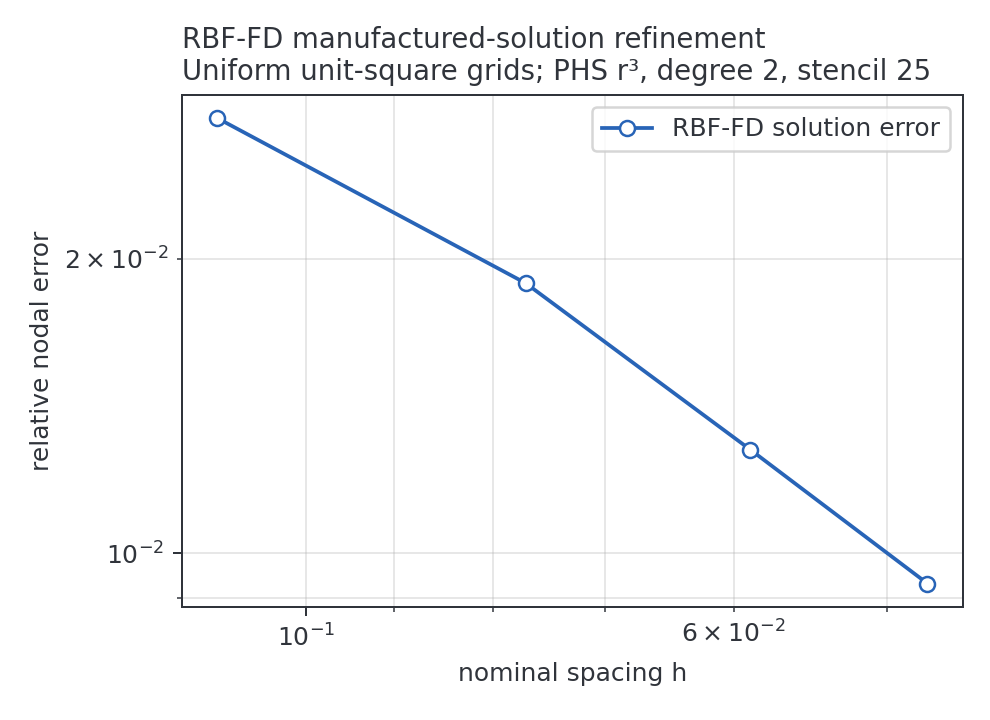
\includegraphics[width=0.72\textwidth]{figures/discretization_convergence.png}
\caption{Manufactured-solution convergence for the verified Poisson discretization.}
\label{fig:disc}
\end{figure}

The first preconditioning system used $N=324$, the same $s=25$ stencil, seed-7 jitter of 0.15, restart 40, tolerance $10^{-9}$, and a 500-step cap.  Its relative discretization error was $5.57\times10^{-3}$, its matrix had 6,468 nonzeros, and its symmetry defect was 0.180.  \Cref{tab:classical} shows why ILU had to remain the reference.  The smaller-stencil construction reduced iterations but its prototype assembly and factorization cost dominated the solve.

\begin{table}[H]
\centering
\caption{Classical baselines on the $N=324$ jittered system.}
\label{tab:classical}
\begin{tabularx}{\textwidth}{Xrrrr}
\toprule
Method & Iterations & Setup (s) & Solve (s) & Total (s) \\
\midrule
No preconditioner & 122 & 0 & 0.0327 & 0.0327 \\
$\operatorname{ILU}(A)$ & 5 & 0.00172 & 0.000763 & 0.00248 \\
Smaller-stencil $B_{13}$ with $\operatorname{ILU}(B_{13})$ & 12 & 0.0385 & 0.00128 & 0.0397 \\
\bottomrule
\end{tabularx}

\end{table}

The next hierarchy varied resolution, jitter, stencil size, scalar coefficient contrast, and ILU budget one factor at a time. Across 15 systems with $N=93$--800, strong ILU required only 5--11 iterations. This was an important negative result because a learned complement had no realistic room to improve most early tests. Scaling to $N=20{,}164$ preserved that conclusion. At the largest size, $A$ occupied 5.691 MiB, ILU occupied 15.289 MiB with fill ratio 2.696, setup took 0.299 s, and the median solve required 19.5 iterations. Assembly, at 3.294 s, was the dominant one-system cost.

\begin{table}[H]
\centering
\caption{Scale-only RBF--FD systems with $s=25$, seed-7 jitter 0.15, and unchanged strong ILU.}
\label{tab:scale}
\resizebox{\textwidth}{!}{\begin{tabular}{rrrrrrrr}
\toprule
$N$ & nnz & $A$ MiB & assembly (s) & ILU setup (s) & ILU MiB & fill & iterations \\
\midrule
2,500  & 57,796  & 0.671 & 0.386 & 0.024 & 1.594 & 2.380 & 9.0 \\
5,041  & 119,305 & 1.385 & 0.798 & 0.050 & 3.588 & 2.600 & 11.0 \\
10,000 & 240,496 & 2.790 & 1.594 & 0.121 & 7.481 & 2.690 & 14.0 \\
20,164 & 490,564 & 5.691 & 3.294 & 0.299 & 15.289 & 2.696 & 19.5 \\
\bottomrule
\end{tabular}
}
\end{table}

\begin{figure}[H]
\centering
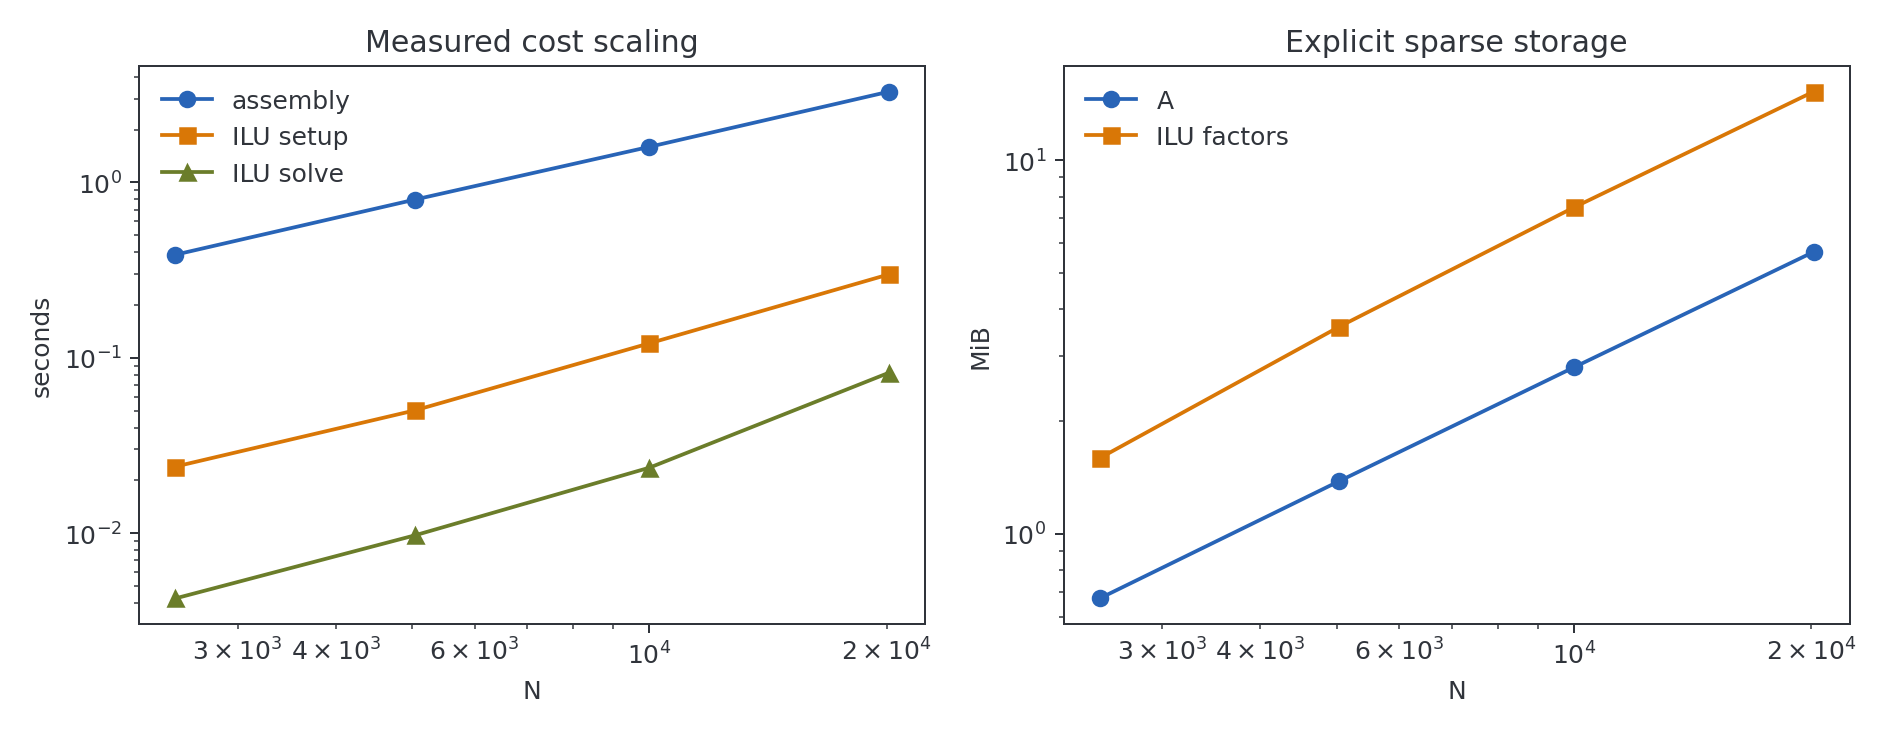
\includegraphics[width=0.86\textwidth]{figures/scale_cost_and_memory.png}
\caption{Assembly, ILU setup, online solve, and sparse-storage scaling.  No scale-only ILU memory wall appears by $N\simeq20{,}000$.}
\label{fig:scale}
\end{figure}

Smooth scalar contrast through $10^4$, a localized contrast-$10^3$ inclusion, and valid centre refinement also remained easy.  In contrast, the standard SPD tensor obtained by rotating eigenvalues $(1,R)$ by $30^\circ$ created a sharp transition.  At $R=100$ and 1000, ILU reached the 300-step cap even though the direct manufactured-solution errors were 0.0142 and 0.00153.  This was the first regime in which the discretization remained meaningful while the strong classical solve was genuinely difficult.

\begin{table}[H]
\centering
\caption{PDE difficulty at $N=5{,}041$.  A reported value of 300 is a cap hit, not an inferred converged count.}
\label{tab:pde}
\resizebox{\textwidth}{!}{\begin{tabularx}{\textwidth}{Xrrrrrr}
\toprule
System & Contrast & Symmetry defect & Conditioning proxy & ILU iterations & Solve (s) & Disc. error \\
\midrule
Smooth scalar & $10$ & 0.087 & $2.64\times10^2$ & 11.0 & 0.009 & $5.48\times10^{-4}$ \\
Smooth scalar & $10^4$ & 0.078 & $1.81\times10^4$ & 10.5 & 0.008 & $2.0\times10^{-3}$ \\
Local scalar & $10^3$ & 0.069 & $5.05\times10^6$ & 11.0 & 0.011 & $1.2\times10^{-2}$ \\
Rotated tensor & $R=10$ & 0.129 & $1.23\times10^4$ & 10.0 & 0.008 & $5.57\times10^{-4}$ \\
Rotated tensor & $R=100$ & 0.139 & $4.51\times10^7$ & 300 cap & 0.397 & $1.42\times10^{-2}$ \\
Rotated tensor & $R=1000$ & 0.140 & $2.08\times10^8$ & 300 cap & 0.459 & $1.53\times10^{-3}$ \\
\bottomrule
\end{tabularx}
}
\end{table}

\begin{figure}[H]
\centering
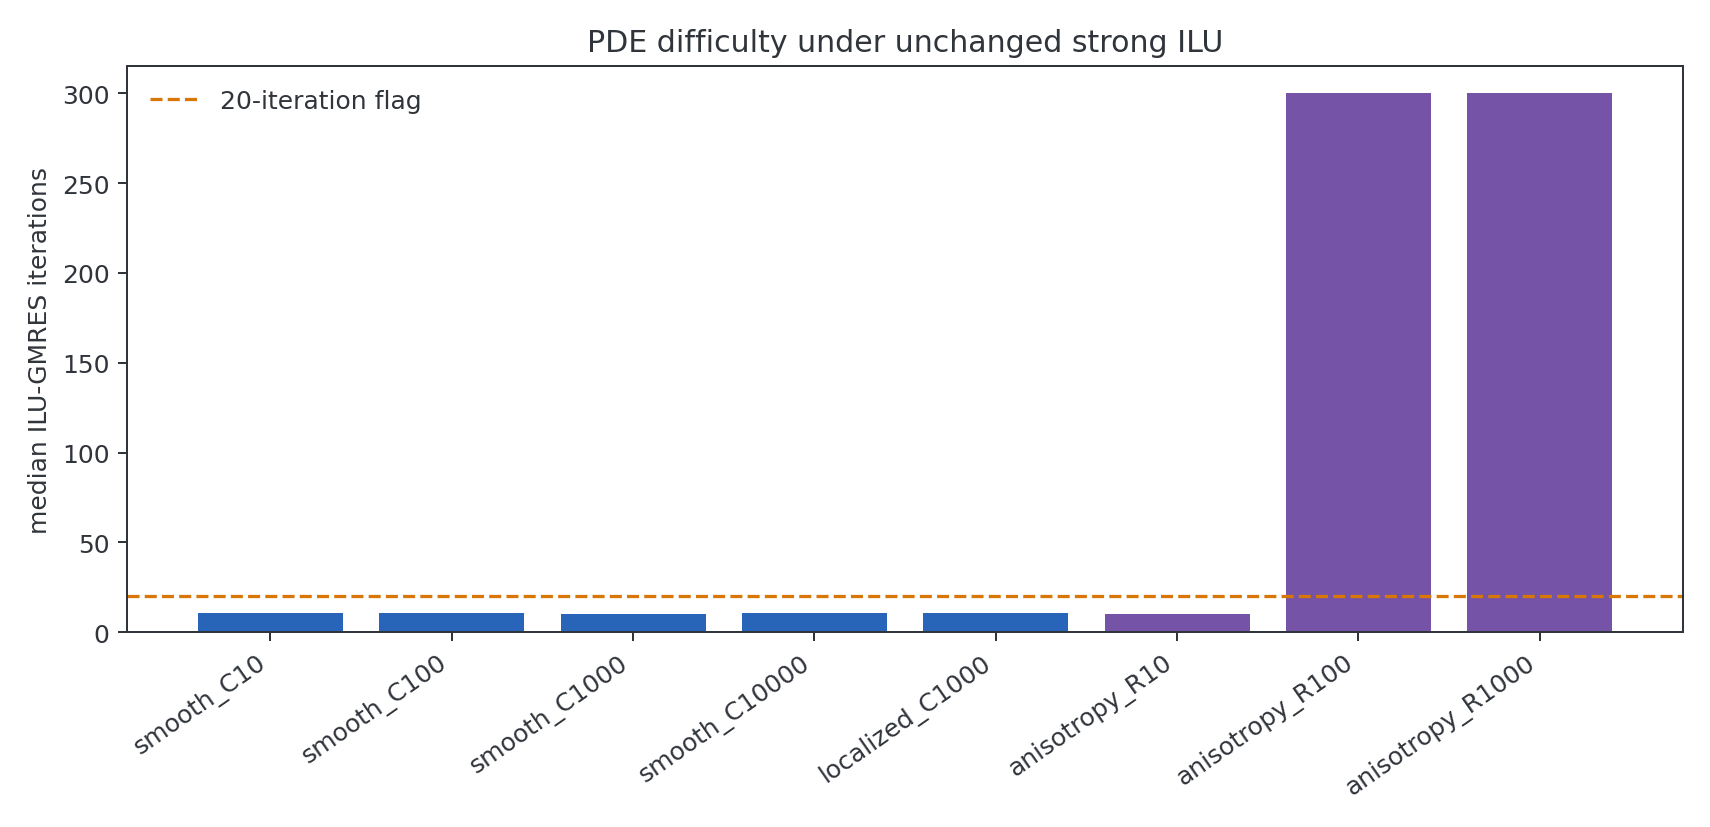
\includegraphics[width=0.88\textwidth]{figures/pde_difficulty.png}
\caption{Strong-ILU behavior under scalar contrast, localized contrast, and rotated anisotropy.}
\label{fig:pde}
\end{figure}

\section{Residual action and first recycle-space evidence}

The validated discretization revealed that strong ILU already solved most regimes cheaply. The next experiments ask what inverse action remains unresolved and whether it has a useful low-dimensional structure. On the initial easy Poisson system, 48 training corrections and 24 held-out corrections mixed synthetic samples with actual GMRES histories. At $q=5$, POD captured 96.5\% of snapshot energy, while mean held-out error was 0.211. At $q=8$, energy reached 99.0\% and mean error fell to 0.179. The classical solve already required only five iterations. POD at $q=20$ reduced one representative solve to four, while a random rank-20 control remained at five. The added setup could not improve total time. Approximate low rank alone did not create a useful preconditioner.

The broader one-factor study reinforced the distinction.  Joint correction snapshots often had $q_{95}\le4$, yet held-out errors reached 0.584 and fifteen high-energy cases produced no Krylov gain.  Across those systems, captured energy and actual iteration reduction had Spearman correlation 0.745, but high energy alone was not sufficient.  \Cref{fig:correctioncurves} shows the normalized spectra, captured energy, and held-out projection curves on the harder family.

\begin{figure}[H]
\centering
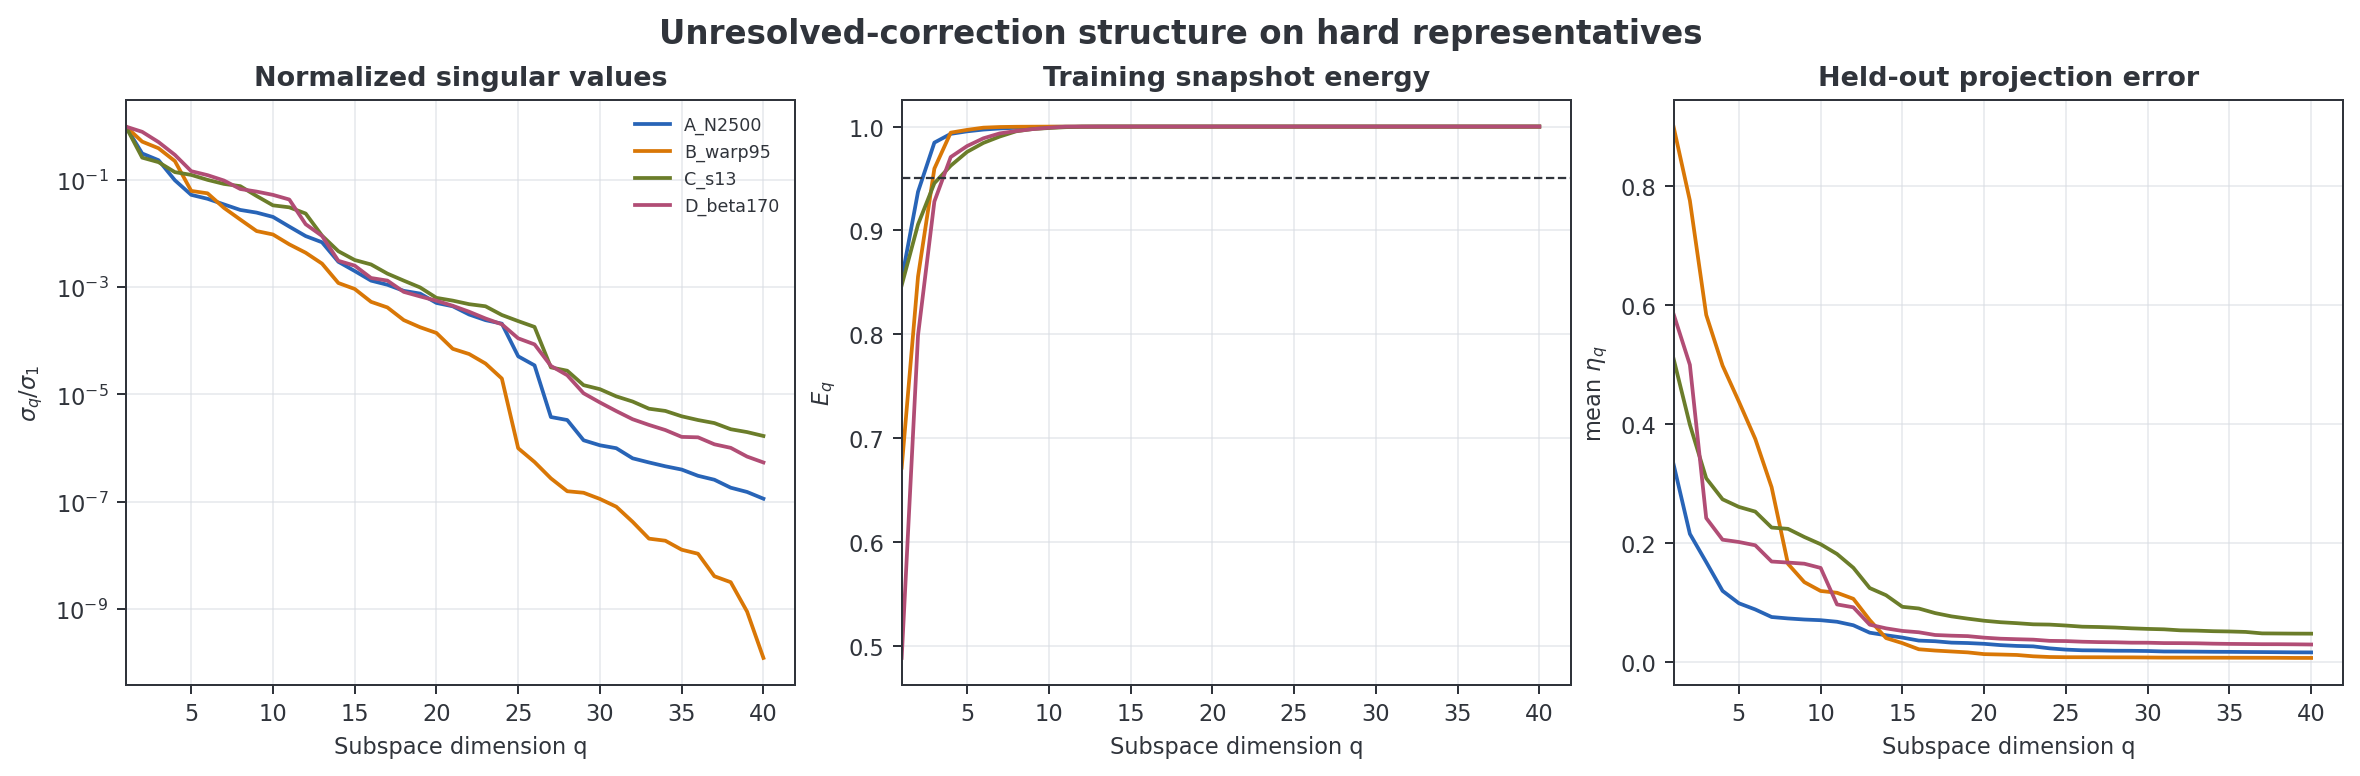
\includegraphics[width=0.93\textwidth]{figures/unresolved_correction_curves.png}
\caption{Unresolved-correction POD diagnostics.  Held-out projection, rather than training energy alone, determines whether low-dimensional evidence is credible.}
\label{fig:correctioncurves}
\end{figure}

When the systems became large or anisotropic, low dimensionality ceased to persist uniformly. Several training snapshot matrices reached 95\% energy with two to five modes, while only the $R=100$ anisotropy case passed the held-out criterion. The $R=1000$ case had $q_{95}=3$ with held-out error 0.790. Scale $N=20{,}164$ had $q_{95}=5$ with held-out error 0.439. The tiny ratios $q/N$ therefore failed to identify an exploitable space.

\begin{table}[H]
\centering
\caption{Correction-POD dimensionality on selected nontrivial or setup-sensitive systems.}
\label{tab:correction}
\begin{tabularx}{\textwidth}{Xrrrrr}
\toprule
System & $N$ & $q_{95}$ & $q_{95}/N$ & held-out $\eta_{95}$ & Structured at 95\%? \\
\midrule
Scale $N=20{,}164$ & 20,164 & 5 & $2.48\times10^{-4}$ & 0.439 & no \\
Smooth scalar $10^4$ & 5,041 & 2 & $3.97\times10^{-4}$ & 0.478 & no \\
Centre refined & 5,041 & 2 & $3.97\times10^{-4}$ & 0.837 & no \\
Rotated anisotropy $R=100$ & 5,041 & 2 & $3.97\times10^{-4}$ & 0.041 & yes \\
Rotated anisotropy $R=1000$ & 5,041 & 3 & $5.95\times10^{-4}$ & 0.790 & no \\
\bottomrule
\end{tabularx}

\end{table}

POD was next compared with Krylov-derived spaces. On the scale-only $N=20{,}164$ system, a rank-16 ordinary Ritz oracle reduced 20 iterations to 10. Smooth scalar contrast $10^4$ improved from 11 to 6 and a valid centre-refined system from 12 to 7. These iteration reductions began from easy solves and did not justify learning. The decisive result was rotated anisotropy at $R=100$: rank-24 correction POD reduced the capped baseline to 99 iterations, whereas rank-24 Ritz reduced it to 48, an 84\% observed reduction. At $R=1000$, neither construction converged by rank 24. Ritz information became the main diagnostic target because it was more solver relevant in the one hard positive regime.

\section{Paired projection for nonsymmetric systems}

The previous section found the first decisive recycle-space benefit in rotated anisotropy. Using that space correctly requires a nonsymmetric construction and a fair comparison of persistent correction with Krylov recycling. Across $R=85$--120, $\norm{A-A\trans}_F/\norm{A}_F$ was 0.138--0.139. A 48-probe estimate for the right-preconditioned operator gave
$\norm{AM^{-1}-(AM^{-1})\trans}_F/\norm{AM^{-1}}_F$ between 1.297 and 1.625. A later verification confirmed that the hard-regime code already used the $AZ=WR$ minimum-residual Petrov construction. Rebuilt rank-eight actions reproduced all earlier iterations exactly, and the historical, explicit Petrov, and recycling-normalized actions agreed to relative error at most $2.29\times10^{-15}$.

The fixed protocol used $N=5{,}041$, $s=25$, node seed 7, jitter 0.15, rotation $30^\circ$, ILU drop tolerance $10^{-3}$ and fill 5, restart 50, tolerance $10^{-8}$, and cap 300.  The oracle came from a 64-step construction trajectory with seed 20261001 and was evaluated on RHS seeds 20261101--20261103.  \Cref{tab:ab,fig:ab} compare persistent Petrov correction with fixed-space recycled GMRES using exactly the same $Z$.  Iterations are identical at every $R$.  Recycling avoids a reduced solve at every preconditioner application and has the lower median online time, with persistent/recycling ratio 1.26.

\begin{table}[H]
\centering
\caption{Same-system rank-eight oracle comparison.  Times are median online wall-clock measurements.}
\label{tab:ab}
\resizebox{\textwidth}{!}{\begin{tabular}{rrrrrrr}
\toprule
$R$ & ILU & Persistent PG & Recycling & PG time (s) & Recycle time (s) & Convergence \\
\midrule
85  & 87  & 32  & 32  & 0.041 & 0.037 & 1.00 \\
90  & 148 & 35  & 35  & 0.051 & 0.049 & 1.00 \\
95  & 148 & 36  & 36  & 0.051 & 0.045 & 1.00 \\
100 & 300 & 78  & 78  & 0.114 & 0.087 & 1.00 \\
105 & 290 & 71  & 71  & 0.102 & 0.081 & 1.00 \\
110 & 300 & 84  & 84  & 0.147 & 0.100 & 1.00 \\
120 & 300 & 298 & 298 & 0.468 & 0.326 & 1.00 \\
\bottomrule
\end{tabular}
}
\end{table}

\begin{figure}[H]
\centering
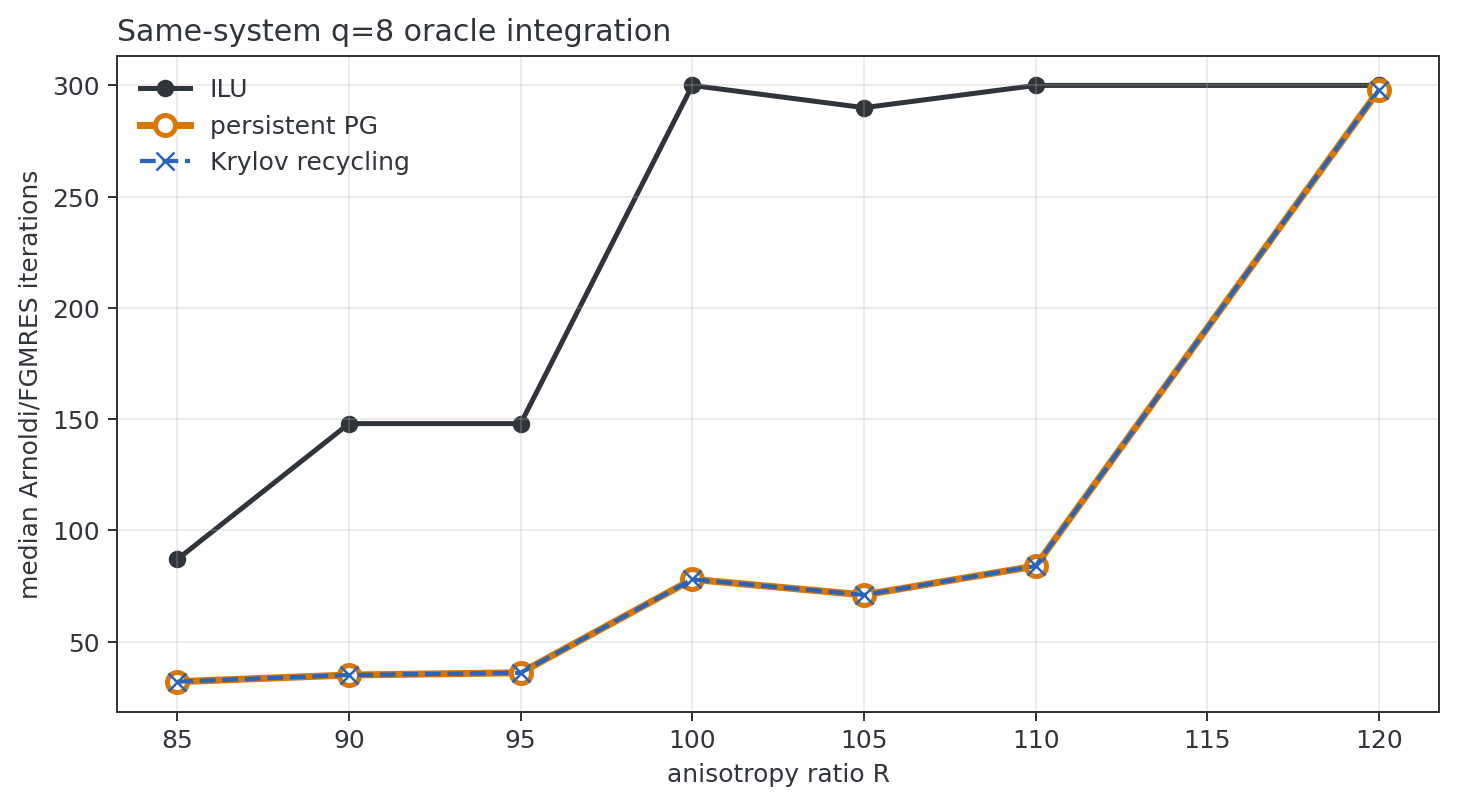
\includegraphics[width=0.83\textwidth]{figures/persistent_vs_recycling.png}
\caption{Persistent Petrov--Galerkin and recycled GMRES exploit the same oracle information and match in iteration count.}
\label{fig:ab}
\end{figure}

The residual-space component explains why one-time correction was insufficient. In the persistent method, the median $\norm{W\trans r_1}/\norm{r_1}$ after the first application was 0.454 at $R=90$, 0.485 at $R=100$, and 0.669 at $R=110$. Each coarse correction reduced it to roundoff. Projected Arnoldi kept the corresponding true-residual component near $4.22\times10^{-10}$ in median. Applying the persistent correction only every fifth preconditioner call cost 14 extra median iterations, and applying it only at initialization cost 121. Repeated enforcement is material, and the Krylov projector supplies it more efficiently.

\begin{figure}[H]
\centering
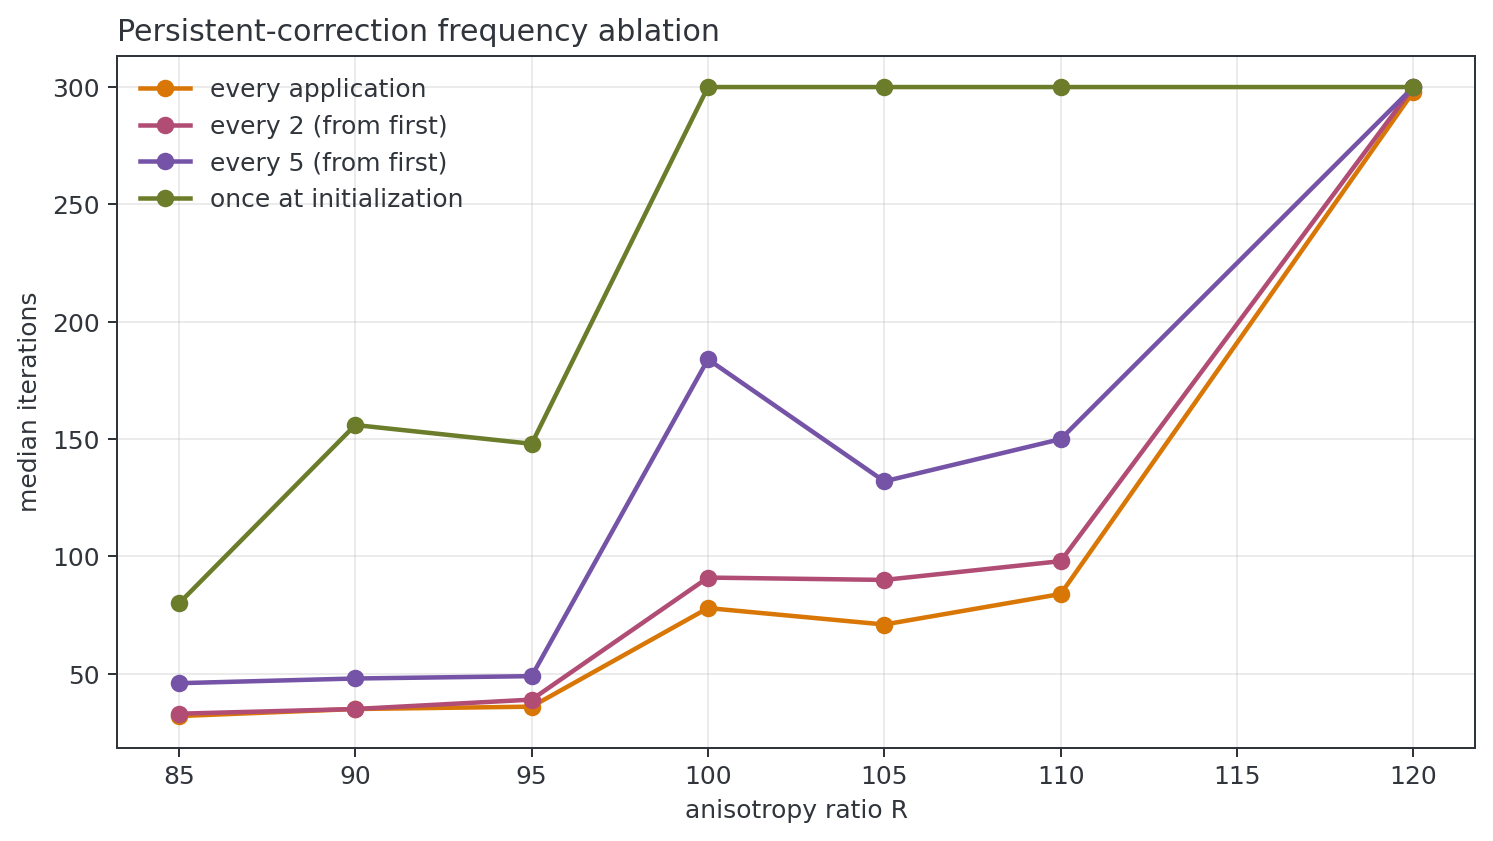
\includegraphics[width=0.82\textwidth]{figures/correction_frequency.png}
\caption{Frequency ablation for the rank-eight Petrov correction.  A single initialization does not reproduce persistent enforcement.}
\label{fig:frequency}
\end{figure}

This relationship is close in spirit to the projected invariant-space mechanism of NeurKItt \citep{luo2024neurkitt}: a conventional preconditioner remains active while a predicted space guides Krylov projection. The RBF--FD question asks whether the space represents a persistent low-dimensional failure of a strong, application-specific ILU and can be predicted or updated economically. The scientific contribution must therefore lie in identifying and predicting that failure space.

\section{Transferability of the first Ritz oracle}

The paired recycle method can exploit an effective oracle space. The unresolved question is whether the first rank-eight Ritz spaces form stable targets across nearby systems. Fine sampling over $R=60$--140 exposed a transition rather than a uniformly hard family. Own-system medians included $148\to35$ at $R=90$, $300\to78$ at $R=100$, and $300\to84$ at $R=110$. At $R=120$, the same construction gave only $300\to298$, and it failed at 130 and 140. Across the hard ratios, median reduction was 65.9\% and convergence was 0.83. \Cref{fig:ritzq} shows that the solver-critical dimension and onset of benefit depend on $R$.

\begin{figure}[H]
\centering
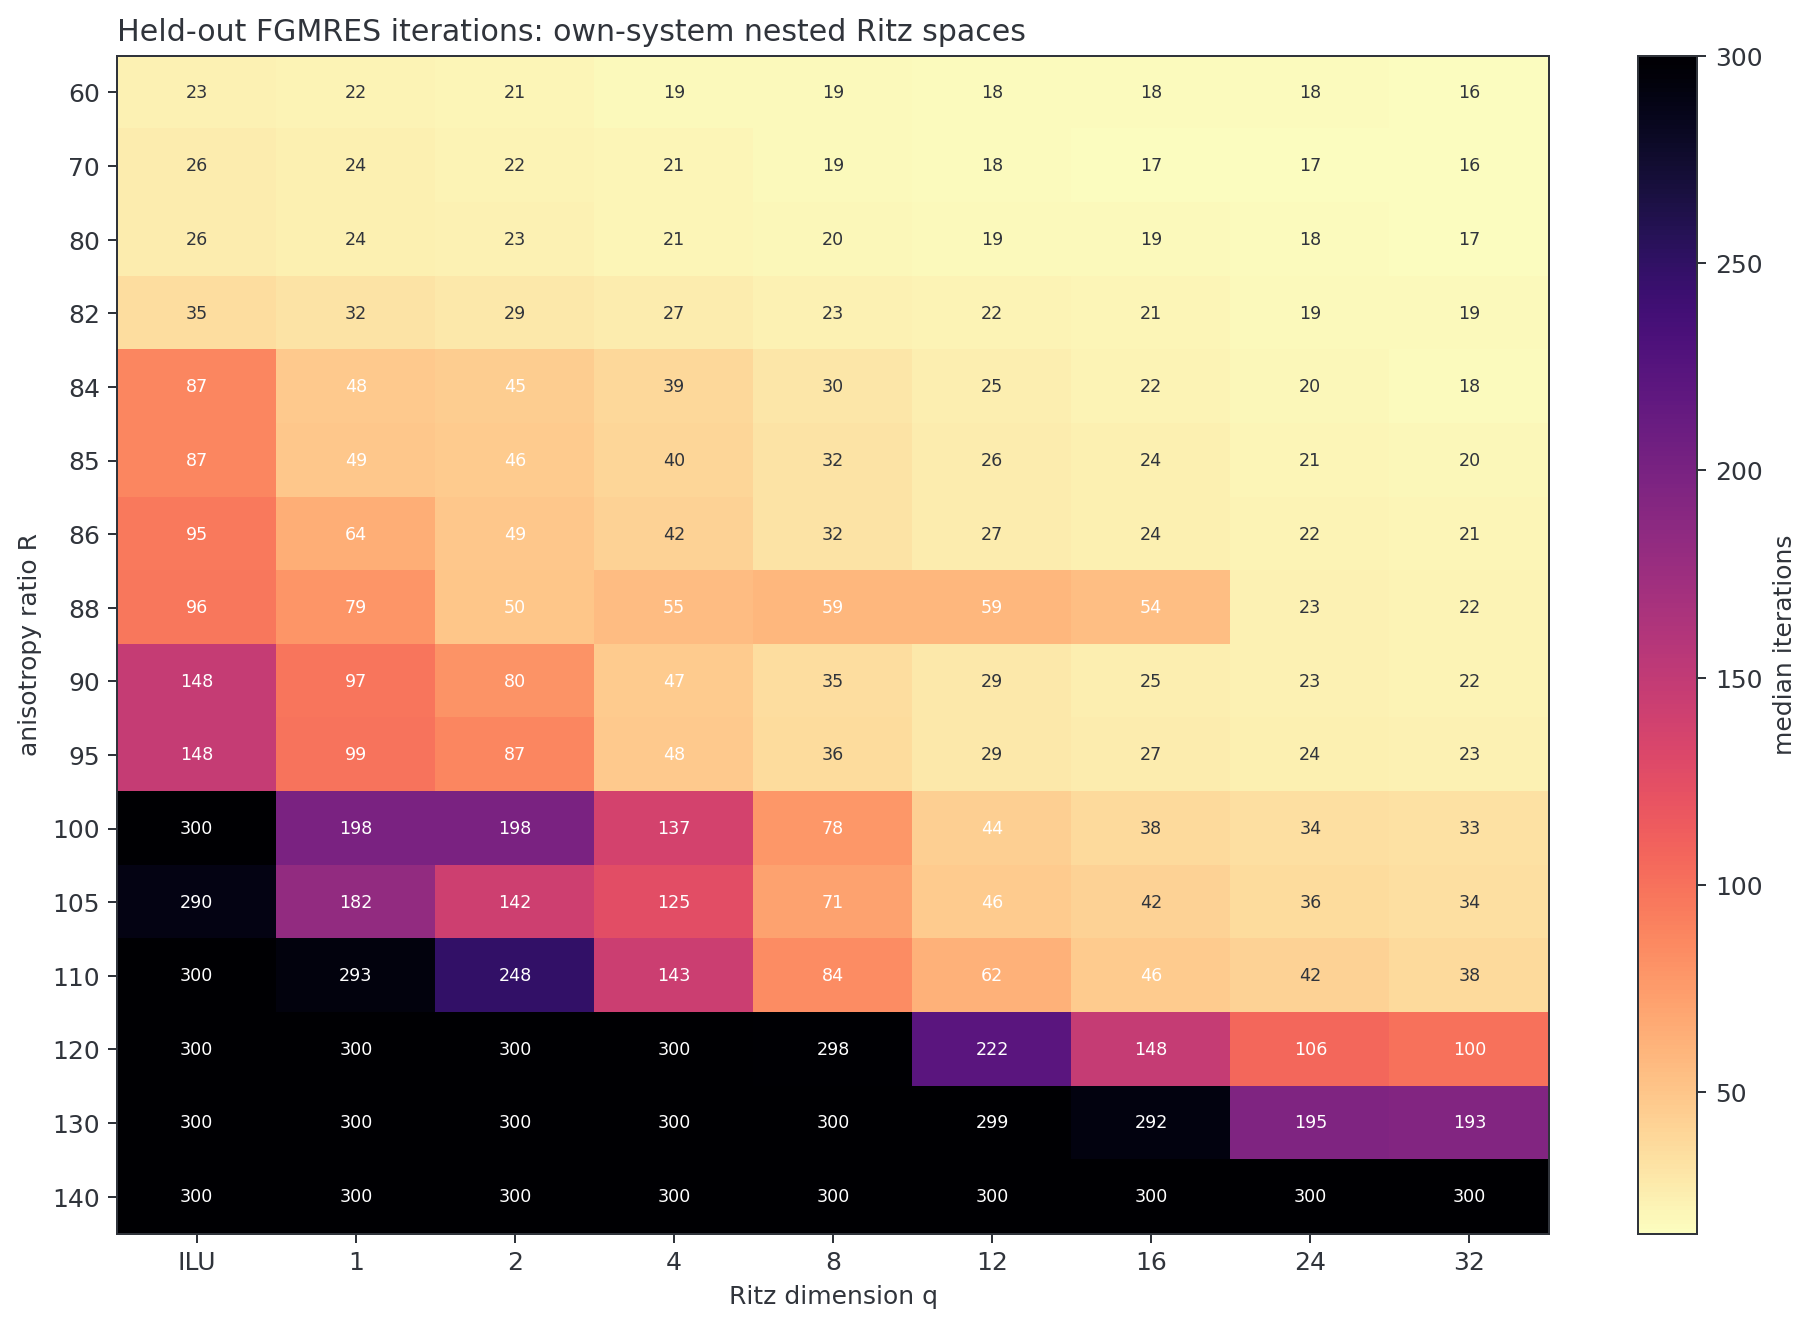
\includegraphics[width=0.90\textwidth]{figures/ritz_q_sweep.png}
\caption{Median iteration count versus anisotropy and Ritz dimension.  A fixed small dimension does not cover the full transition.}
\label{fig:ritzq}
\end{figure}

The system-specific spaces varied systematically in aggregate but were not stable enough for supervised labels.  For rank eight, all-pair normalized projector distance had median 0.787, local pairs with $|\Delta R|\le2$ had median 0.488, and the median maximum principal angle was $87.4^\circ$.  Distance in $R$ and projector distance had Spearman correlation 0.884.  Nearby reuse retained useful iteration reductions on several pairs, but its hard-regime convergence rate was 0.75 and its median gap to the own oracle was four iterations.  Small node perturbations were substantially more damaging than changing the construction RHS.

Tracking individual Ritz directions did not find a globally stable mode.  Completing complex conjugate planes reduced neighboring projector distance only from 0.558 to 0.537.  Spectral-gap clustering produced no block that was simultaneously stable and solver critical.  Low-rank cluster matches had normalized distance 0.845, six clusters were critical, and none also passed the stability gate.  Slightly enlarged crossing blocks improved own-system reduction to 68.8\% but left neighboring reuse at 75\% convergence.  Thus the instability was not merely an arbitrary rotation inside a clearly stable rank-eight invariant block.

Transfer also separated right-space information from the test-space partner.  Reusing $Z_i$ while rebuilding $A_jZ_i=W_{j\leftarrow i}R_{j\leftarrow i}$ gave, for example, $300\to100$ on $95\to100$ and $290\to94$ on $100\to105$, compared with own-oracle counts 78 and 71.  Full donor-pair reuse and target-recomputed $W$ behaved similarly.  Because the target-side $W$ was already recomputed in the main transfer, poor high-$R$ transfer cannot be blamed on symmetric coupling or reuse of the wrong residual partner.

Finally, 142 controlled spaces and 426 held-out solves tested whether a geometric or short-rollout objective predicts actual acceleration.  The solution-space projector metric had Spearman correlation $-0.205$ with relative iteration reduction.  The residual-space metric $d_W$ was stronger overall at $-0.840$, but aligned in only two of four perturbation families and had leave-family-out prediction correlation 0.394.  Ten-step residual ratio had correlation $-0.497$ and also reversed ranking on the random-perturbation family.  No metric passed the cross-family reliability gate.

\begin{figure}[H]
\centering
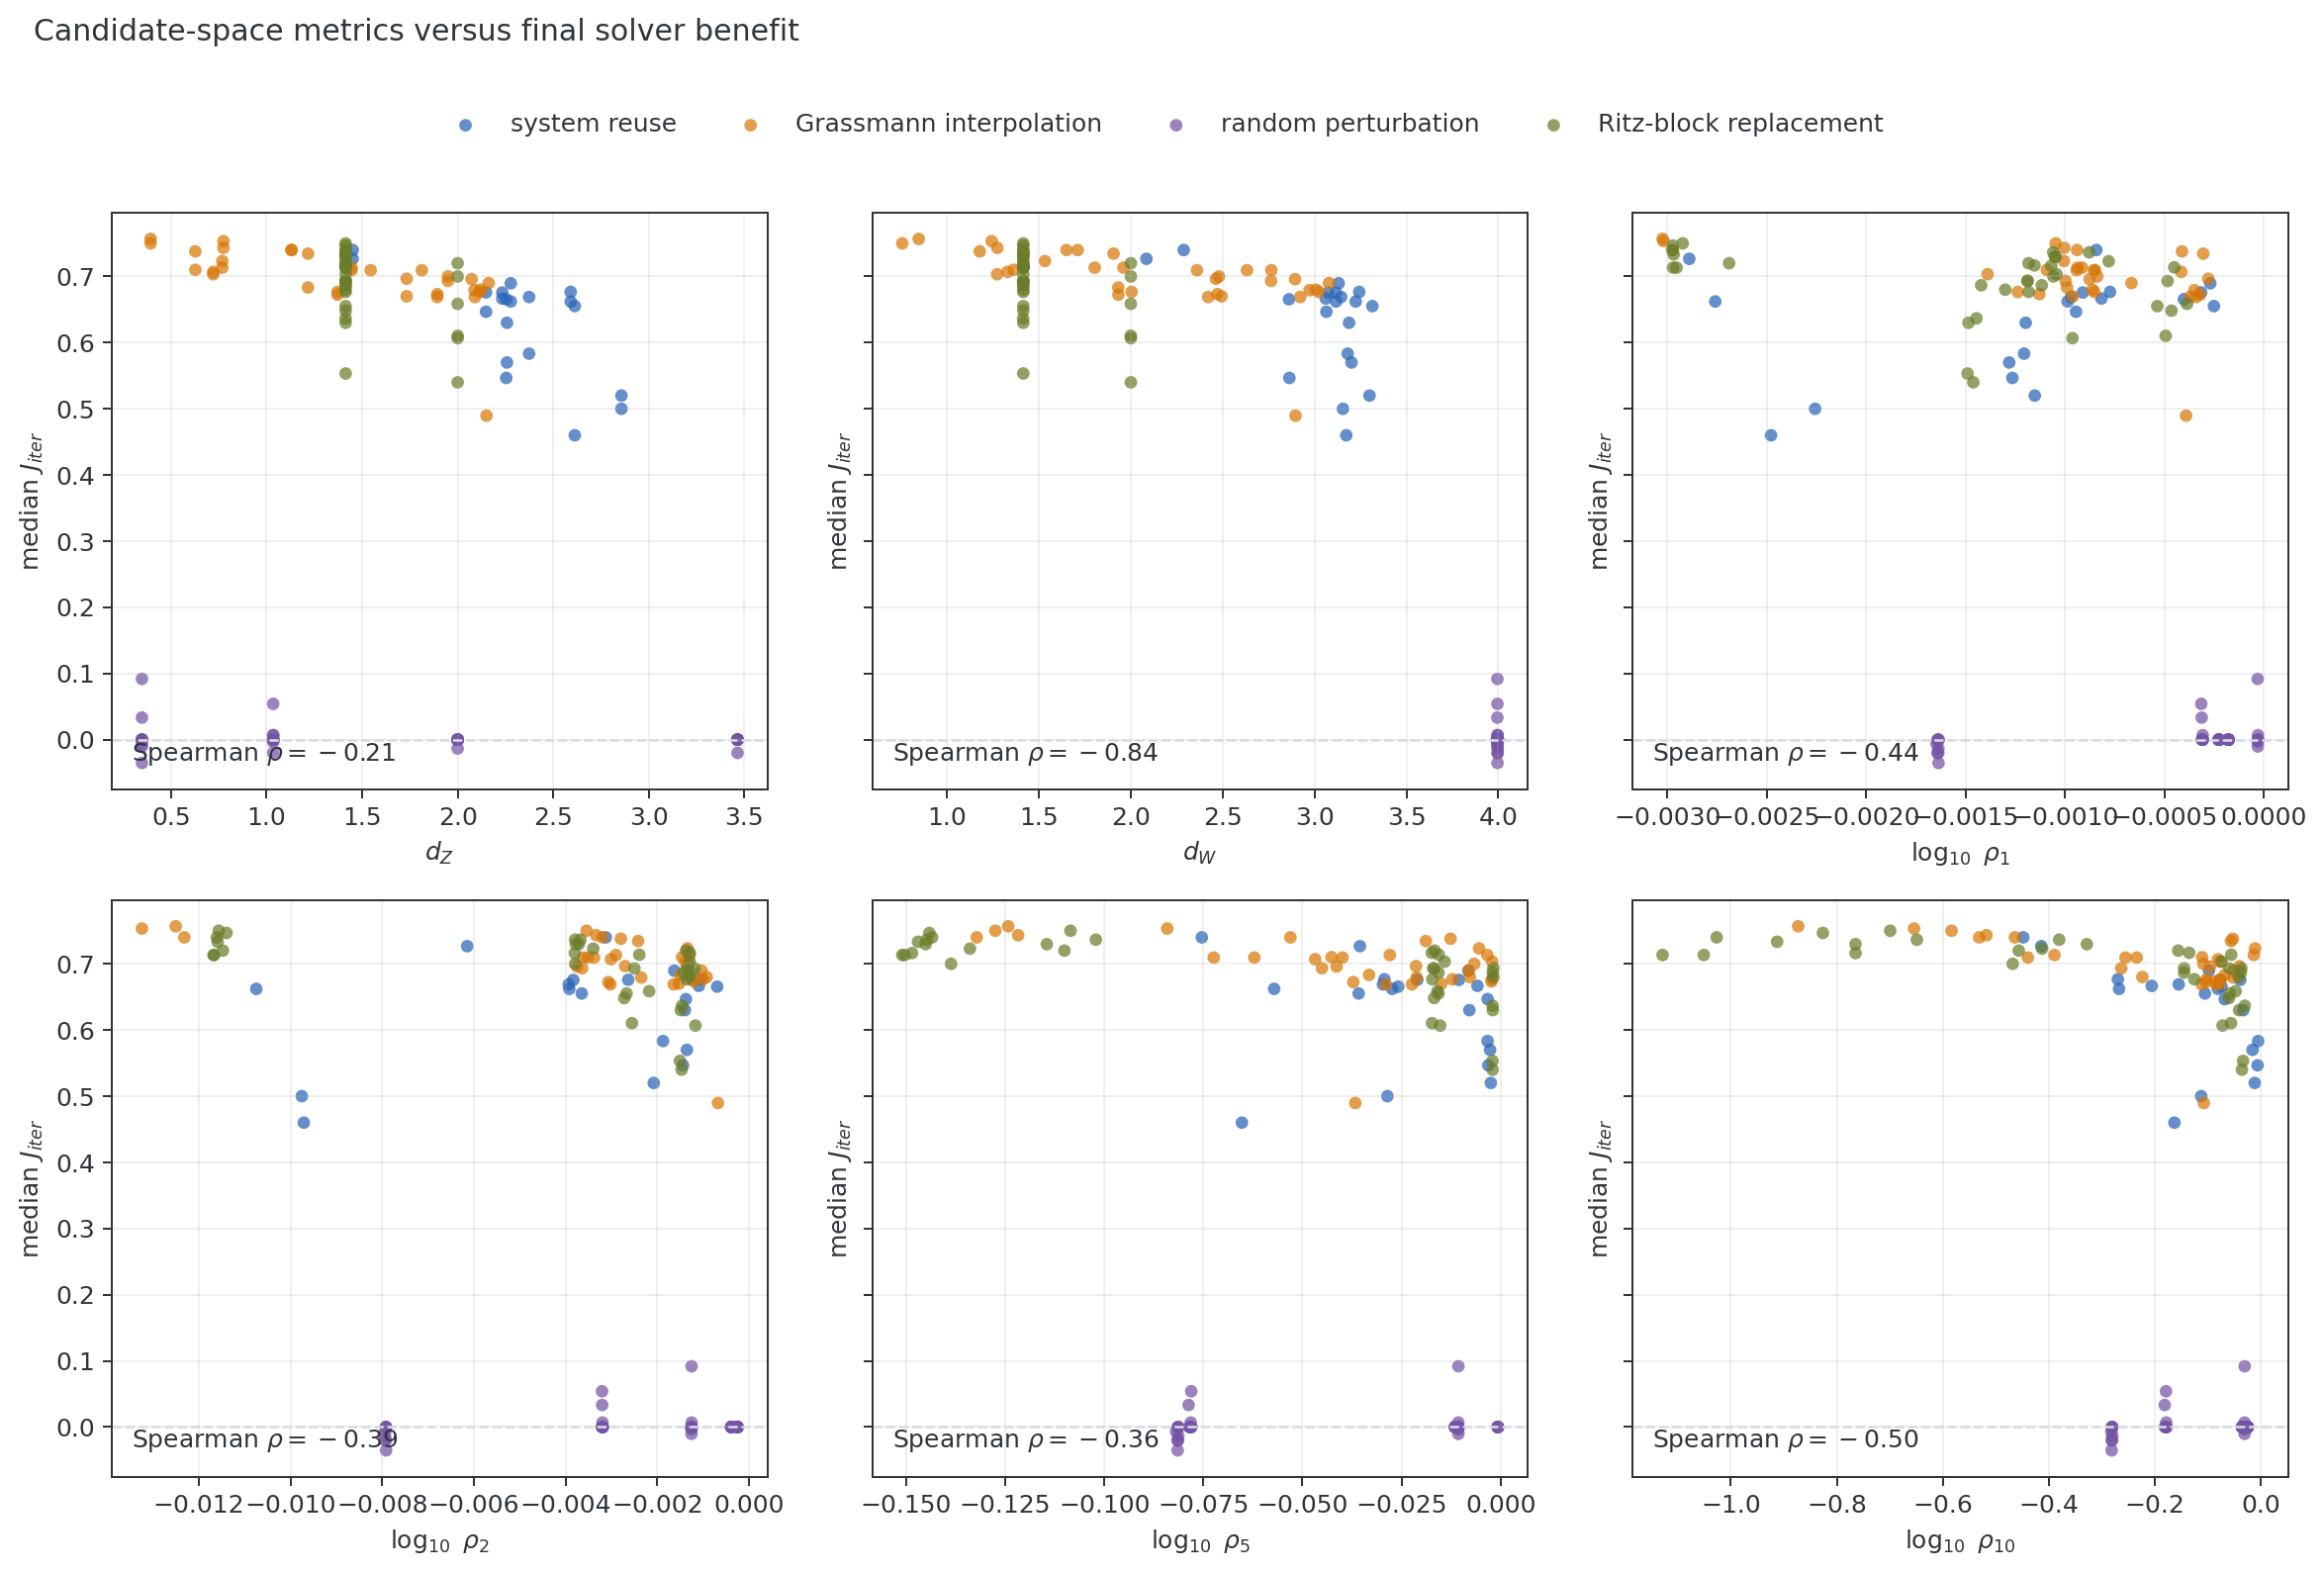
\includegraphics[width=0.95\textwidth]{figures/metric_vs_solver_benefit.png}
\caption{Projector and short-horizon metrics against final iteration reduction.  Residual-space geometry is the strongest aggregate diagnostic but not a reliable universal target.}
\label{fig:targets}
\end{figure}

Geometry and solver value can disagree sharply.  A donor $R=90$ space used at $R=100$ had $d_Z=2.591$ and $d_W=3.243$, yet reduced the capped baseline to 97 iterations, giving observed $J_{\rm iter}=0.677$.  Conversely, controlled perturbations with favorable geometric rank were not uniformly favorable in the solver.  Projector similarity is therefore neither necessary nor sufficient for the desired ranking.

\section{Direct correction learning}

The unstable first Ritz labels motivated a return to direct correction learning, which avoids a fixed low-rank assumption. This branch preserved \cref{eq:missing}. The initial fixed-$N=900$ MLP took a residual and compact system parameters and predicted the full missing correction. It used one hidden layer of width 64 and 116,228 parameters. On actual solver directions, its median relative error and magnitude ratio were both approximately 996, and all 12 learned solves reached the 800-step cap.

The diagnostic pipeline was then corrected.  Actual vectors presented to the ILU preconditioner during Arnoldi were collected on disjoint train, validation, and test trajectories.  Homogeneous normalization used $\widehat v=v/\norm v_2$ and trained against $d(v)/\norm v_2$, with inference $d_\theta(v)=\norm v_2N_\theta(\widehat v,\xi)$.  On held-out ILU trajectories the MLP error fell to 0.770, its norm ratio was 0.923, and cosine similarity was 0.786.  After insertion into FGMRES, however, the model changed the Krylov trajectory.  The median nearest-training cosine fell from 0.653 offline to 0.159, closed-loop correction error rose to 2.519, and the norm ratio rose to 2.525.  All six MLP solves hit 300 iterations.

A small two-layer, width-16 message-passing GNN used coordinates, normalized vector value, boundary flag, coefficient, stencil edges, relative coordinates, distances, and RBF--FD weights.  It had only 3,521 parameters and was permutation equivariant to $2.20\times10^{-16}$, whereas the MLP equivariance defect was 2.98.  Graph structure repaired the ordering defect, but not the solver.  The GNN required 134 median iterations and 0.813 s, compared with 11 iterations and 0.0098 s for ILU.

Three rounds of on-policy aggregation stabilized the MLP under its own trajectory: the undamped model moved from no convergence at a 120-step diagnostic cap to 67 iterations with full convergence.  Damping $\alpha d_\theta$ with $\alpha=0.1$ reduced the median to 14, and the norm limiter was inactive in the median case.  This was a post-hoc mechanism diagnostic, not a deployment result.  It remained slower than the 11-iteration, 0.0084-s ILU reference and required 0.020 s online, excluding 18.4 s of training.  The GNN remained unreliable.  \Cref{tab:direct,fig:direct} summarizes why the direct branch was paused.

\begin{table}[H]
\centering
\caption{Direct-complement development.  Caps and convergence denominators differ according to the declared experiment and are retained explicitly.}
\label{tab:direct}
\small
\begin{tabularx}{\textwidth}{>{\raggedright\arraybackslash}p{0.20\textwidth}>{\raggedright\arraybackslash}X>{\centering\arraybackslash}p{0.10\textwidth}>{\centering\arraybackslash}p{0.09\textwidth}>{\raggedright\arraybackslash}p{0.16\textwidth}}
\toprule
Experiment and method & Correction diagnostic & Iterations & Conv. & Timing comparison \\
\midrule
Initial direct MLP & solver-direction error $\approx 996$ & 800 cap & $0/12$ & ILU: 11 iterations \\
Solver-aware MLP & offline error 0.770; closed-loop 2.519 & 300 cap & $0/6$ & ILU: 11 iterations \\
Solver-aware GNN & offline error 1.158 & 134 median & $6/6$ & 0.813 s; ILU 0.0098 s \\
On-policy MLP, undamped & on-policy error 1.112 & 67 median & $2/2$ & ILU: 11 iterations \\
On-policy MLP, $\alpha=0.1$ & damped, no clipping in median & 14 median & $4/4$ & 0.020 s; ILU 0.0084 s \\
On-policy GNN & on-policy error 4.464 & 83.5 median & $2/4$ & 0.626 s; ILU 11 iterations \\
\bottomrule
\end{tabularx}

\end{table}

\begin{figure}[H]
\centering
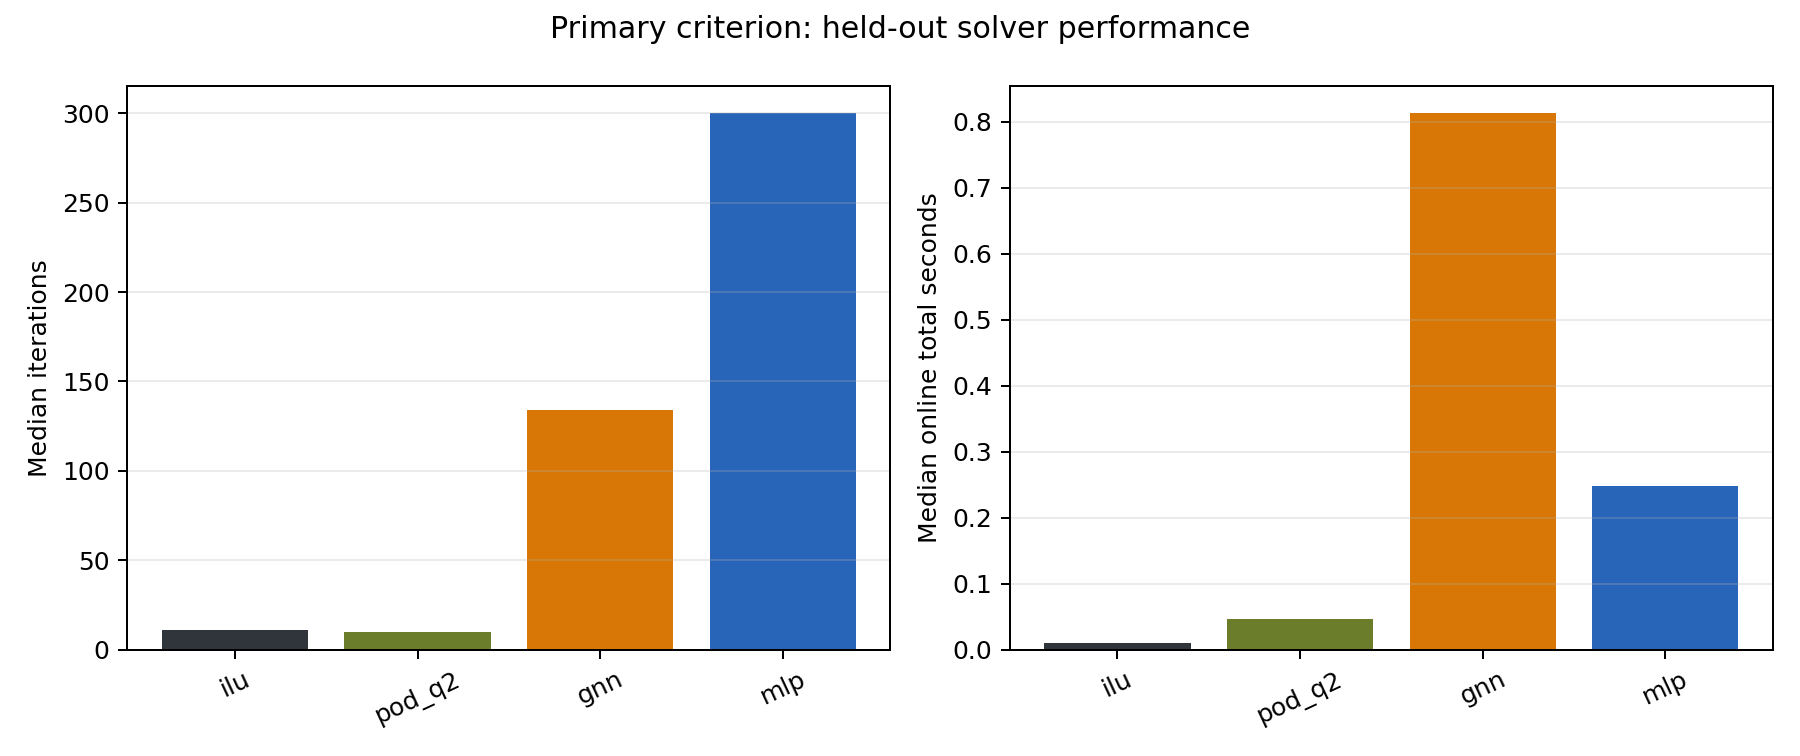
\includegraphics[width=0.74\textwidth]{figures/direct_learning_closed_loop.png}
\caption{Held-out solver comparison after solver-aware training.  Better offline correction metrics did not produce a competitive closed-loop preconditioner.}
\label{fig:direct}
\end{figure}

The target remained $d(v)=A^{-1}v-M^{-1}v$ throughout this branch. Solver-aware sampling fixed the first distribution mismatch, normalization fixed the open-loop scale failure, and on-policy aggregation improved stability. None produced a robust iteration or cost advantage over strong ILU. The evidence gave no reason to increase model size.

\section{Recycle-space learning in controlled families}

Direct correction learning improved under solver-aware training but remained slower and less reliable than ILU. The next experiments return to recycle spaces within controlled parameter families, where label regularity can be tested before increasing input complexity. The first study used one scalar parameter, fixed nodes, and $R\in[90,110]$. Training used even ratios, with disjoint odd-ratio validation and test sets. A training-only $Z$-POD dictionary reached 99.12\% energy at $p=19$. The MLP followed \cref{eq:mlpipeline} and the $W$-projector loss in \cref{eq:wloss}.

The held-out model was solver useful within this restricted family. It converged on every solve and recovered a median 0.939 of the own-oracle iteration reduction. Its normalized $d_W$ remained 0.685, and it needed 89 median iterations. Nearest reuse recovered 0.952 and midpoint Grassmann interpolation 0.983. The learned method matched or improved on nearest reuse for only 20\% of test ratios. Deterministic reuse or interpolation therefore remained stronger within this family.

Changing only the dictionary did not repair the ranking.  At fixed $p=19$, projecting held-out oracles into the original $Z$-POD dictionary produced normalized $W$ error 0.595.  The corresponding errors were 0.700 for the training-only $AZ$-aware dictionary and 0.797 for the joint dictionary.  The best learned arm remained the original dictionary with recovery 0.939.  This ablation also exposed a sign error in the proposed joint reconstruction expression: minimizing a negative weighted error would reward worse $AZ$ reconstruction, so the implementation explicitly used the intended nonnegative plus-weight objective.

Action supervision changed only the loss.  With $AZ=WR$ and $U=ZR^{-1}$, the recycle action on a probe was $c(r)=UW\trans r$.  Training used 7,743 solver-generated probes from training systems, with 2,999 validation and 3,158 test probes.  Median held-out action error improved from 0.935 under $W$ loss to 0.858 under action loss, but the solver worsened from 89 to 98 median iterations and oracle recovery fell from 0.939 to 0.851.  Better average action approximation did not preserve the few directions that controlled convergence.

\begin{table}[H]
\centering
\caption{Fixed-architecture recycle-space learning and ablations.  $\eta=(k_{\rm ILU}-k_{\rm method})/(k_{\rm ILU}-k_{\rm oracle})$ is computed per RHS before aggregation.}
\label{tab:learning}
\small
\begin{tabularx}{\textwidth}{>{\raggedright\arraybackslash}X>{\centering\arraybackslash}p{0.08\textwidth}>{\raggedright\arraybackslash}p{0.24\textwidth}>{\centering\arraybackslash}p{0.12\textwidth}>{\centering\arraybackslash}p{0.11\textwidth}>{\centering\arraybackslash}p{0.13\textwidth}}
\toprule
Family/ablation & Reduced rank $p$ & Main offline metric & Median iterations & Median $\eta$ & Deterministic $\eta$ \\
\midrule
Scalar $R$, $W$-projector MLP & 19 & normalized $d_W=0.685$ & 89 & 0.939 & 0.983 \\
$W$-aware dictionary ablation & 19 & best arm remained $Z$-POD & 89 & 0.939 & 0.983 \\
Scalar $R$, action-loss MLP & 19 & action error $0.935\to0.858$ & 98 & 0.851 & 0.983 \\
Two-parameter $(R,\theta)$ MLP & 27 & normalized $d_W=0.648$ & 47 & 0.921 & 0.855 \\
\bottomrule
\end{tabularx}

\end{table}

The next experiment changed the family rather than the network.  It used a spatially constant tensor
\begin{equation}
 K(R,\theta)=Q(\theta)\begin{bmatrix}R&0\\0&1\end{bmatrix}Q(\theta)\trans,
 \qquad
 Q(\theta)=\begin{bmatrix}\cos\theta&-\sin\theta\\\sin\theta&\cos\theta\end{bmatrix}.
 \label{eq:constanttensor}
\end{equation}
Thus the input was finite dimensional, $(R,\theta)\mapsto Z$. A legacy implementation stored the eigenvalues in the opposite order, so the experiment applied the exact conversion $\phi=\theta-90^\circ$. The maximum tensor mismatch was $3.71\times10^{-16}$.

The hardness scan covered $R\in\{90,95,100,105,110\}$ and physical angles $15^\circ$--$45^\circ$, with extra points from $27^\circ$ to $33^\circ$.  Angles at most $25^\circ$ were easy, while angles at least $33^\circ$ generally capped for both ILU and rank-eight recycling.  Training was therefore restricted, before learning, to the connected transition rectangle $R\in[95,100]$, $\theta\in[30^\circ,31^\circ]$ where both classical difficulty and oracle value existed.

\begin{figure}[H]
\centering
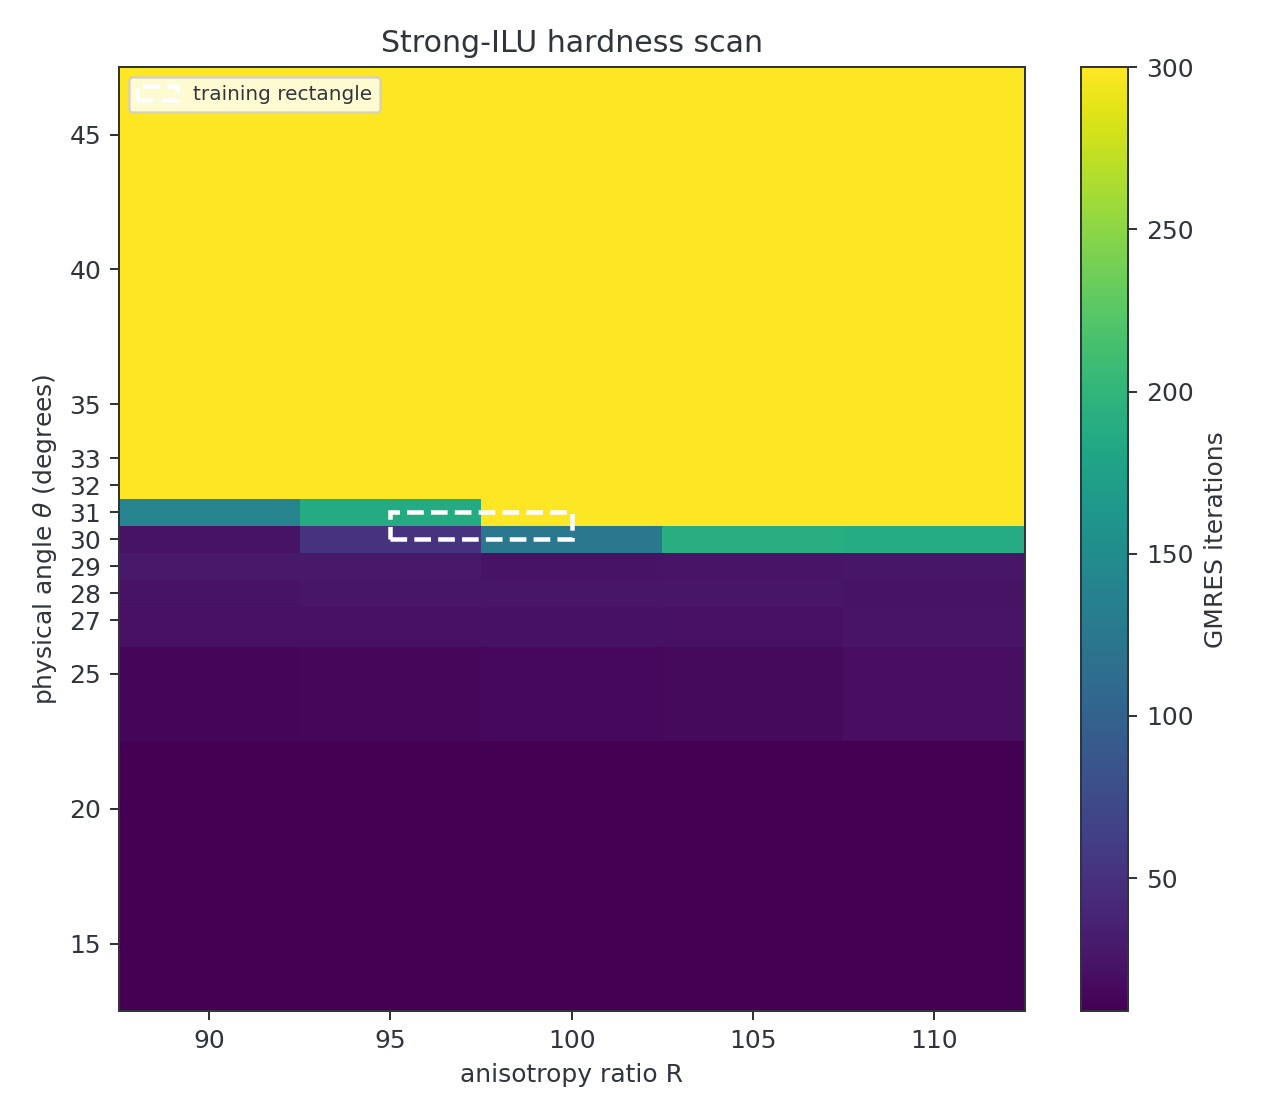
\includegraphics[width=0.88\textwidth]{figures/two_parameter_hardness.png}
\caption{Strong-ILU iteration scan for the spatially constant two-parameter anisotropy tensor.}
\label{fig:twohard}
\end{figure}

The training set was a $5\times5$ tensor grid.  Sixteen cell centres were strictly intermediate in both parameters and were split checkerboard-style into eight validation and eight test systems.  A training-only dictionary reached 99.1\% energy at $p=27$.  The MLP became $2\to64\to128\to216$ and otherwise retained the same optimizer, precision, seeds, and $W$ loss.  Deterministic interpolation followed Grassmann geodesics in both coordinate orders and then took their Grassmann midpoint.

On held-out test systems, the selected MLP achieved median recovery 0.921 versus 0.855 for interpolation, with median iteration difference $-1.5$. The 24 matched RHS solves split 12--12 in wins, the paired Wilcoxon value was $p=0.074$, and median solve-time difference was $-0.001$ s. The methods were computationally comparable. The data do not support significant MLP superiority. This is the strongest learned result in the RBF--FD branch, within a narrow fixed-instance interpolation problem.

\begin{figure}[H]
\centering
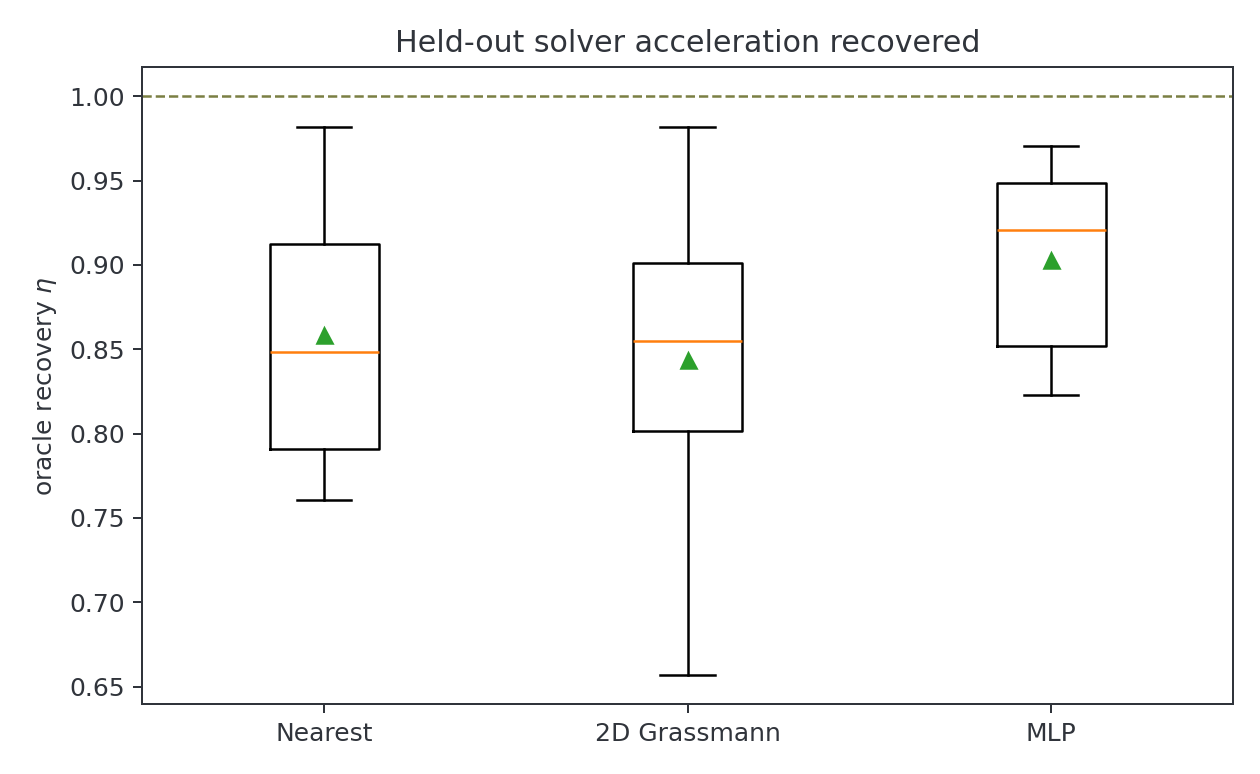
\includegraphics[width=0.73\textwidth]{figures/two_parameter_recovery.png}
\caption{Oracle recovery on the held-out spatially constant $(R,\theta)$ family.  Heterogeneous pointwise wins preclude a superiority claim.}
\label{fig:tworecovery}
\end{figure}

\section{Spatial coefficients break the short fixed-rank oracle}

The controlled families showed that learning can interpolate a validated oracle in a narrow setting. The next experiment replaces the finite-dimensional input with a function-valued tensor field and tests whether the same short fixed-rank oracle survives. The tensor is
\begin{equation}
 K(x,y)=Q(\theta(x,y))\operatorname{diag}(R(x,y),1)Q(\theta(x,y))\trans,
 \label{eq:fieldtensor}
\end{equation}
with
\begin{equation}
\begin{aligned}
 \log R(x,y)&=a_0+a_1\sin(\pi x)+a_2\cos(\pi y)
                 +a_3\sin(\pi x)\cos(\pi y),\\
 \theta(x,y)&=\theta_0+b_1\sin(\pi x)+b_2\cos(\pi y).
\end{aligned}
 \label{eq:fields}
\end{equation}
Thirty-six Latin-hypercube fields used seed 20261901.  The prescribed ranges were
$a_0\in[\log80,\log120]$, $a_1,a_2\in(-0.18,0.18)$, $a_3\in(-0.12,0.12)$, $\theta_0\in(25^\circ,35^\circ)$, and $b_1,b_2\in(-5^\circ,5^\circ)$.  Realized nodewise ratios spanned 69.10--158.77 and angles 19.46--40.94 degrees.  Every field was uniformly SPD and used the exact product-rule operator \cref{eq:variableoperator}.

All 36 discretizations were numerically valid.  Manufactured relative error had median 0.0011 and maximum 0.0087.  Strong-ILU difficulty was heterogeneous: median iteration count across systems was 27.5 with range 16--300, seven systems needed at most 20, fifteen needed at least 50, and fifteen needed at least 100 or capped.  The full distribution was reported before oracle selection.

\begin{figure}[H]
\centering
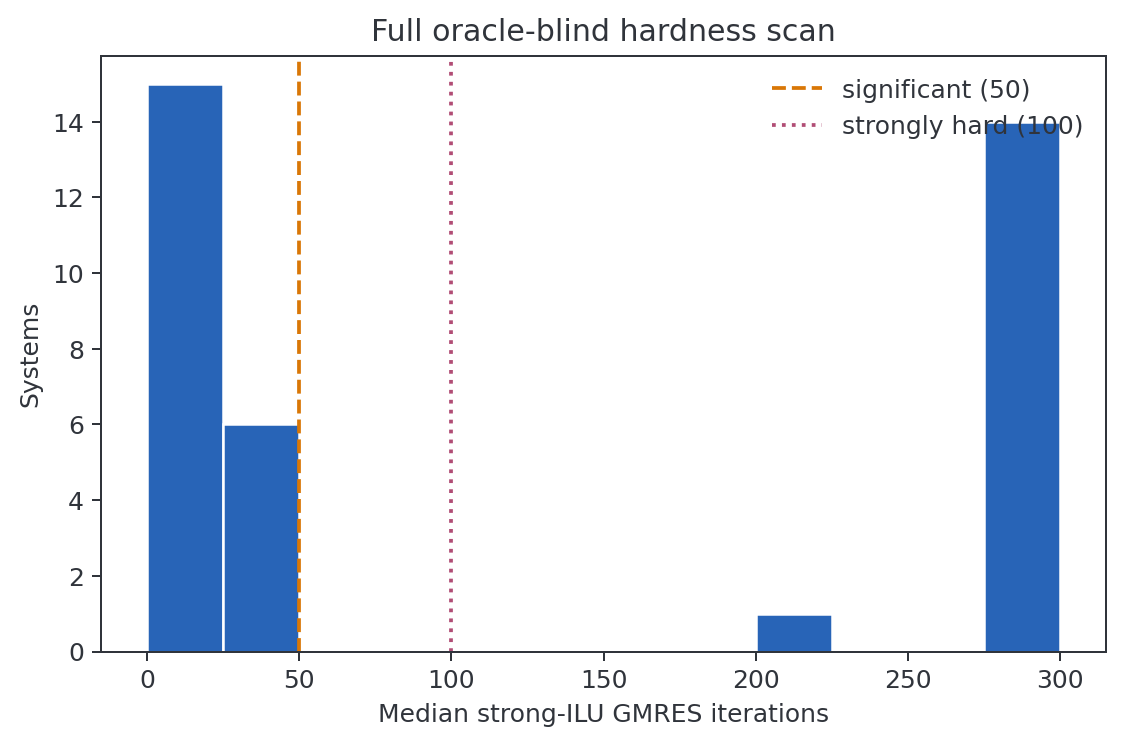
\includegraphics[width=0.74\textwidth]{figures/spatial_field_hardness.png}
\caption{Classical difficulty over the complete 36-field sample.}
\label{fig:fieldhard}
\end{figure}

An 18-system oracle subset was fixed from evenly spaced ILU-difficulty order statistics before any oracle outcome was observed.  Among its eight hard systems, only ID 15 passed the strong rank-eight criterion, improving from 211 to 41 iterations.  The other seven all remained at the 300-step cap.  This failure differs fundamentally from a neural model failing to learn a useful oracle.  No model was trained because the oracle itself was not consistently useful.

\begin{table}[H]
\centering
\caption{Rank-eight own-system Ritz oracle on the eight hard spatial-field systems.}
\label{tab:spatialoracle}
\begin{tabular}{rrrrr}
\toprule
Field ID & ILU iterations & $q=8$ Ritz iterations & $\gamma_{\rm oracle}$ & Oracle convergence \\
\midrule
3  & 300 & 300 & 0.000 & 0.00 \\
7  & 300 & 300 & 0.000 & 0.00 \\
10 & 300 & 300 & 0.000 & 0.00 \\
14 & 300 & 300 & 0.000 & 0.00 \\
15 & 211 & 41  & 0.806 & 1.00 \\
17 & 300 & 300 & 0.000 & 0.00 \\
19 & 300 & 300 & 0.000 & 0.00 \\
34 & 300 & 300 & 0.000 & 0.00 \\
\bottomrule
\end{tabular}

\end{table}

\begin{figure}[H]
\centering
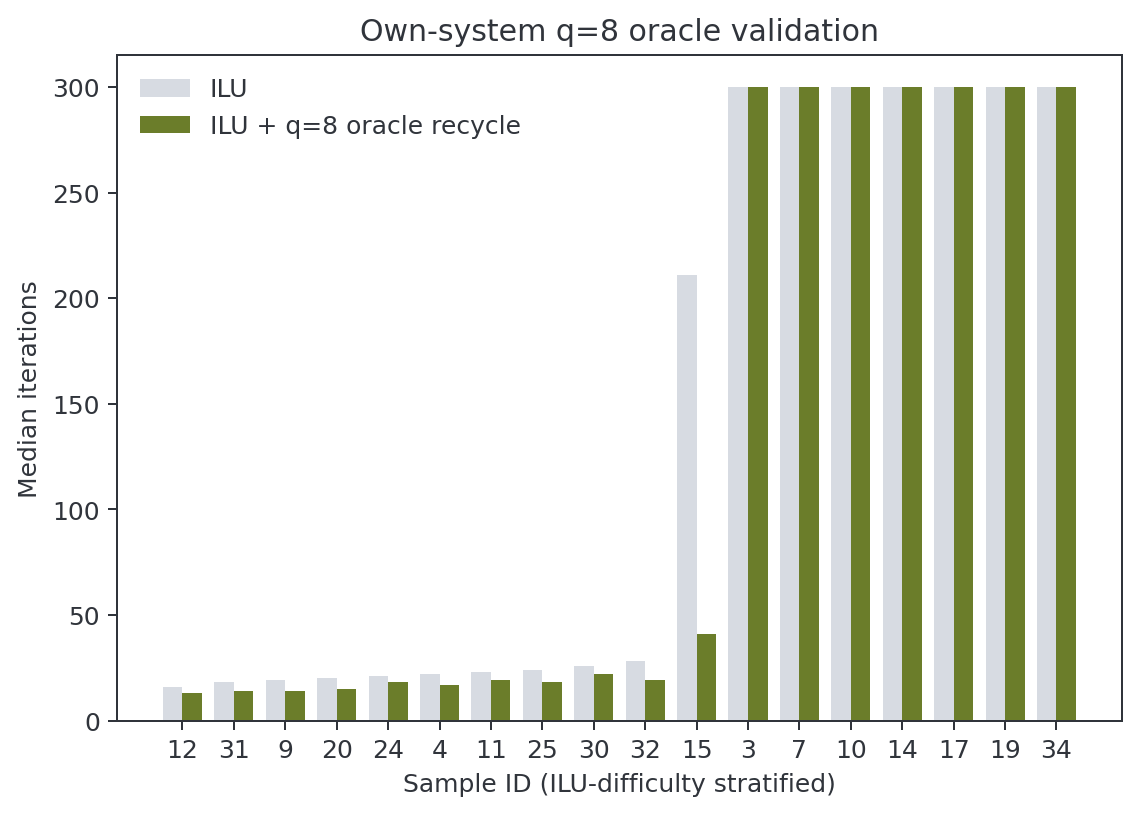
\includegraphics[width=0.78\textwidth]{figures/spatial_field_oracle.png}
\caption{ILU and rank-eight own-oracle iterations across the difficulty-stratified subset.}
\label{fig:fieldoracle}
\end{figure}

The oracle spaces were also more complex as a family.  Concatenated hard-system $Z$ snapshots required dictionary dimensions 30, 43, and 47 for 95\%, 99\%, and 99.5\% energy.  The nearest-field-neighbor normalized projector distance had median 0.825 and the median maximum principal angle was $87.2^\circ$.  Coefficient-field distance did not explain space distance: Spearman correlation was $-0.189$ with $p=0.336$.

A controlled diagnostic changed only oracle dimension and definition on the same eight hard systems. Ordinary smallest-magnitude Ritz was tested through requested rank 32 with invariant pairs preserved. ID 15 passed at rank four, and ID 34 joined only at rank 32 with $300\to150$. ID 14 improved to 225 without reaching the 40\% reduction criterion. IDs 3, 7, 10, and 17 never improved within the first 32 directions. A modest rank increase did not repair the family.

\begin{figure}[H]
\centering
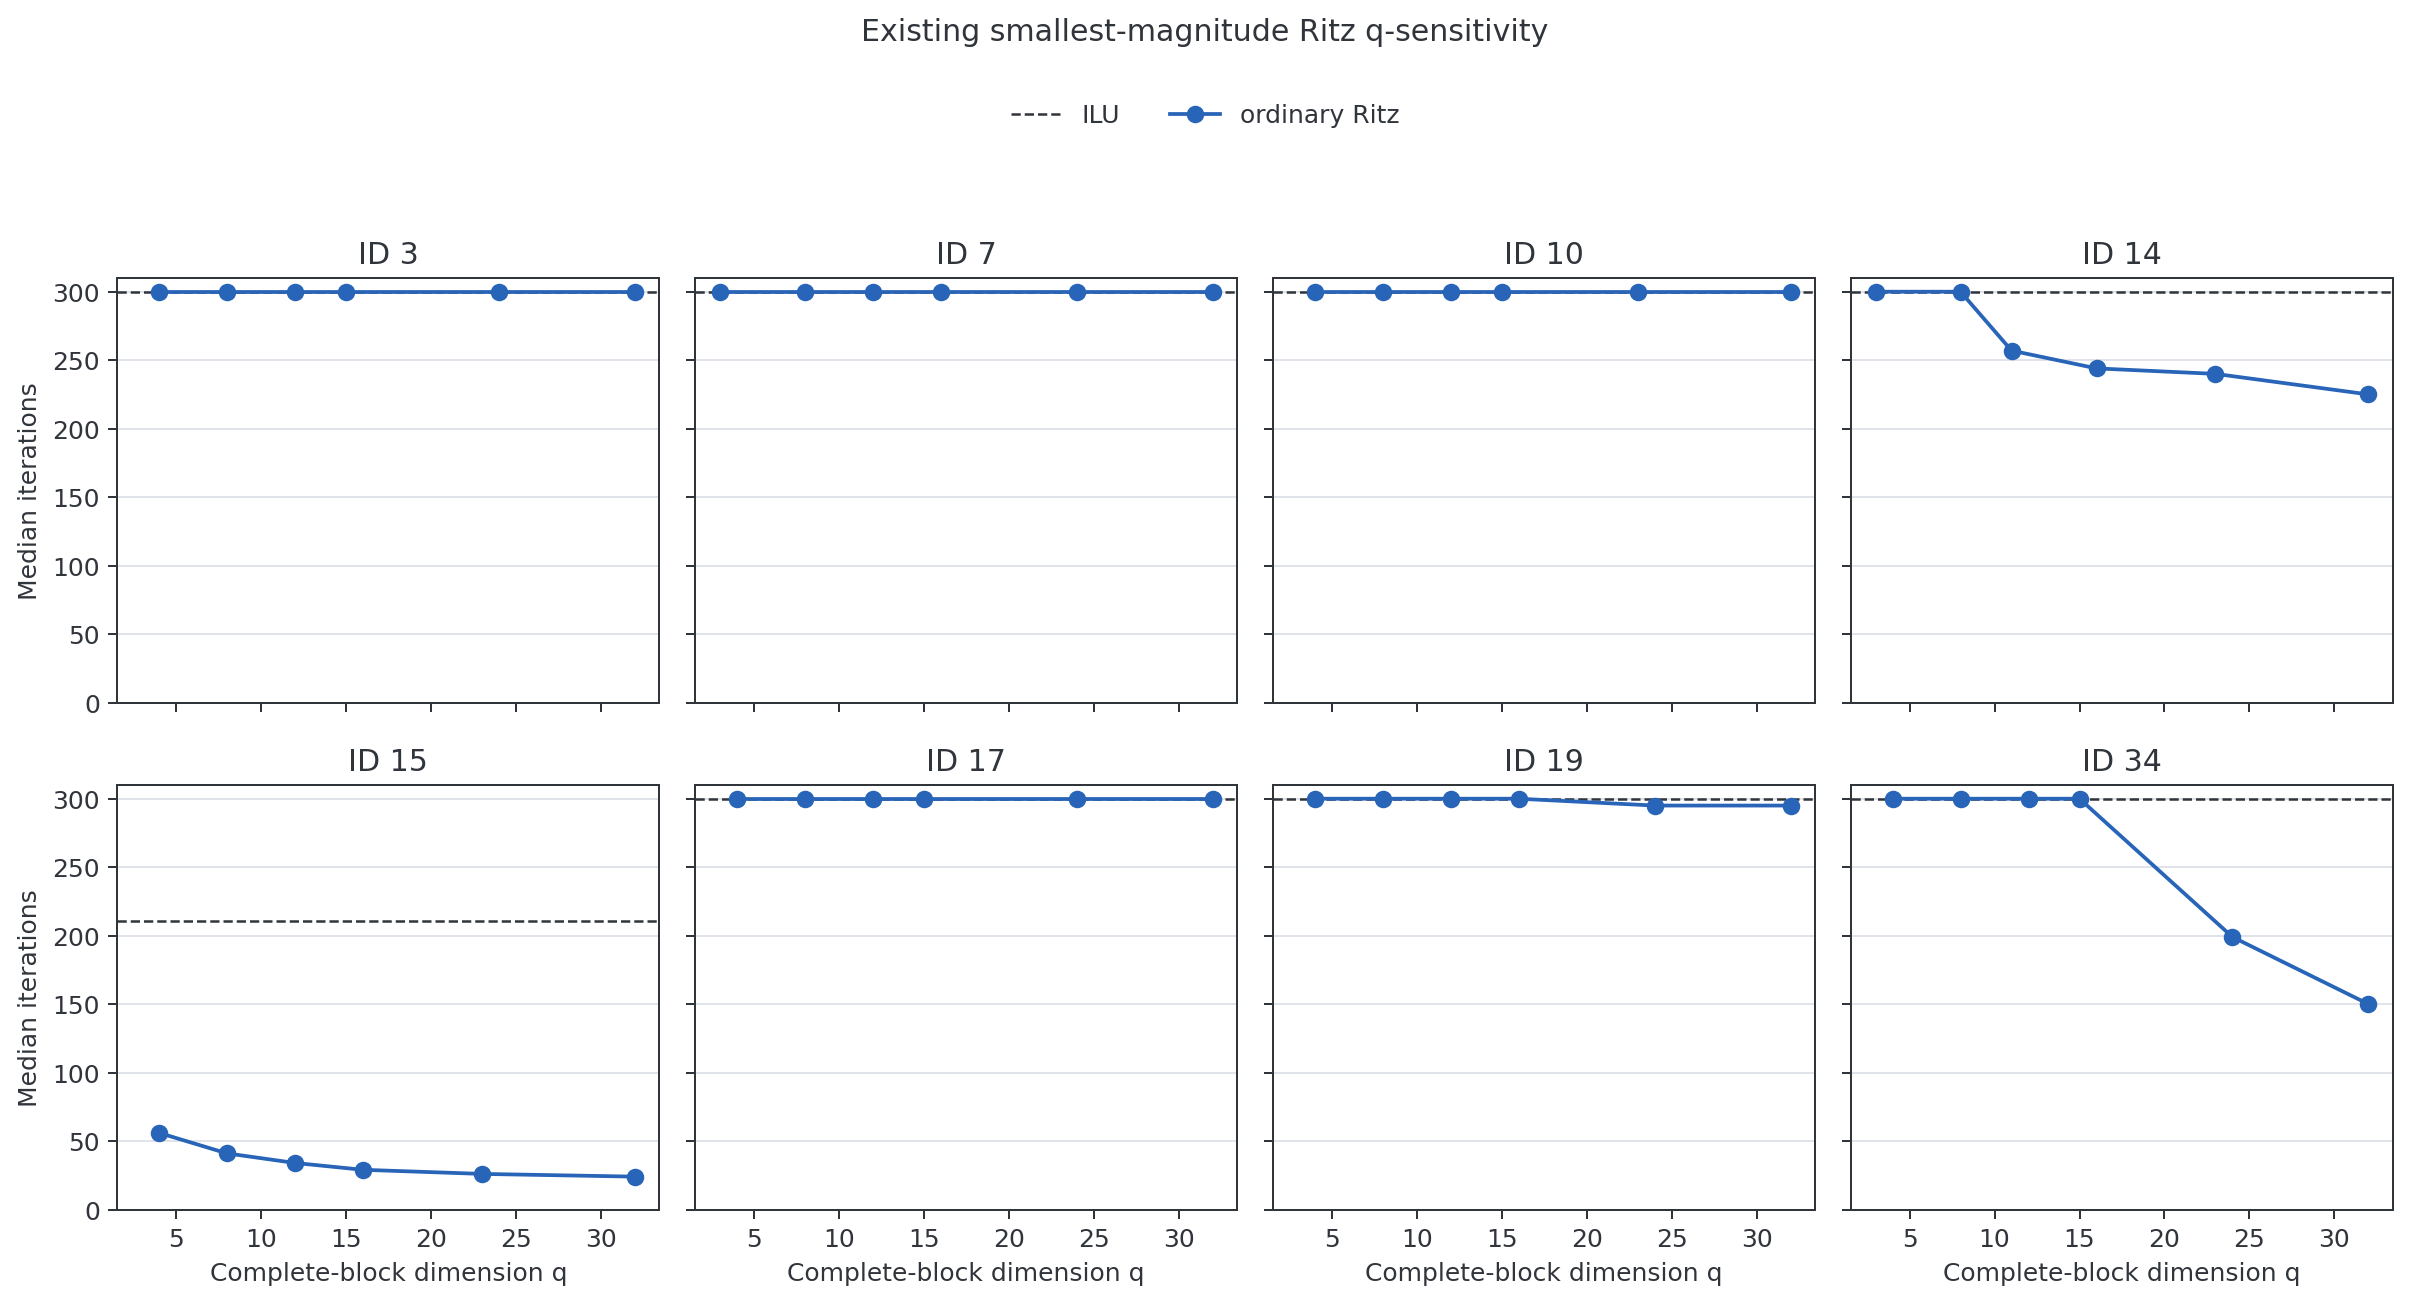
\includegraphics[width=0.91\textwidth]{figures/spatial_q_sensitivity.png}
\caption{Ordinary Ritz q-sensitivity on the eight hard spatial-field systems.}
\label{fig:spatialq}
\end{figure}

Harmonic Ritz used the same 64-step right-preconditioned Arnoldi information and selected values nearest zero. Correction POD used three disjoint construction trajectories, 16 actual preconditioner inputs per trajectory, and the unchanged missing action in \cref{eq:missing}. Ordinary and harmonic Ritz each passed two of eight systems. Correction POD passed one.

\begin{table}[H]
\centering
\caption{Best tested classical diagnostic spaces on the spatial-field family.  Strong success requires all three held-out solves to converge and median reduction at least 40\%.}
\label{tab:spatialdiag}
\small
\begin{tabularx}{\textwidth}{XrrrX}
\toprule
Diagnostic space & Strong successes & Positive control ID 15 & Additional success & Interpretation \\
\midrule
Ordinary Ritz, $q\le32$ & $2/8$ & $211\to24$ at $q=32$ & ID 34: $300\to150$ at $q=32$ & Not a common dimension fix \\
Harmonic Ritz, $q\le32$ & $2/8$ & $211\to25$ at $q=32$ & ID 34: $300\to149$ at $q=32$ & Selection rule does not rescue family \\
Correction POD, $q\le32$ & $1/8$ & $211\to36$ at $q=32$ & none & Compressibility is not recycle relevance \\
\bottomrule
\end{tabularx}

\end{table}

\begin{figure}[H]
\centering
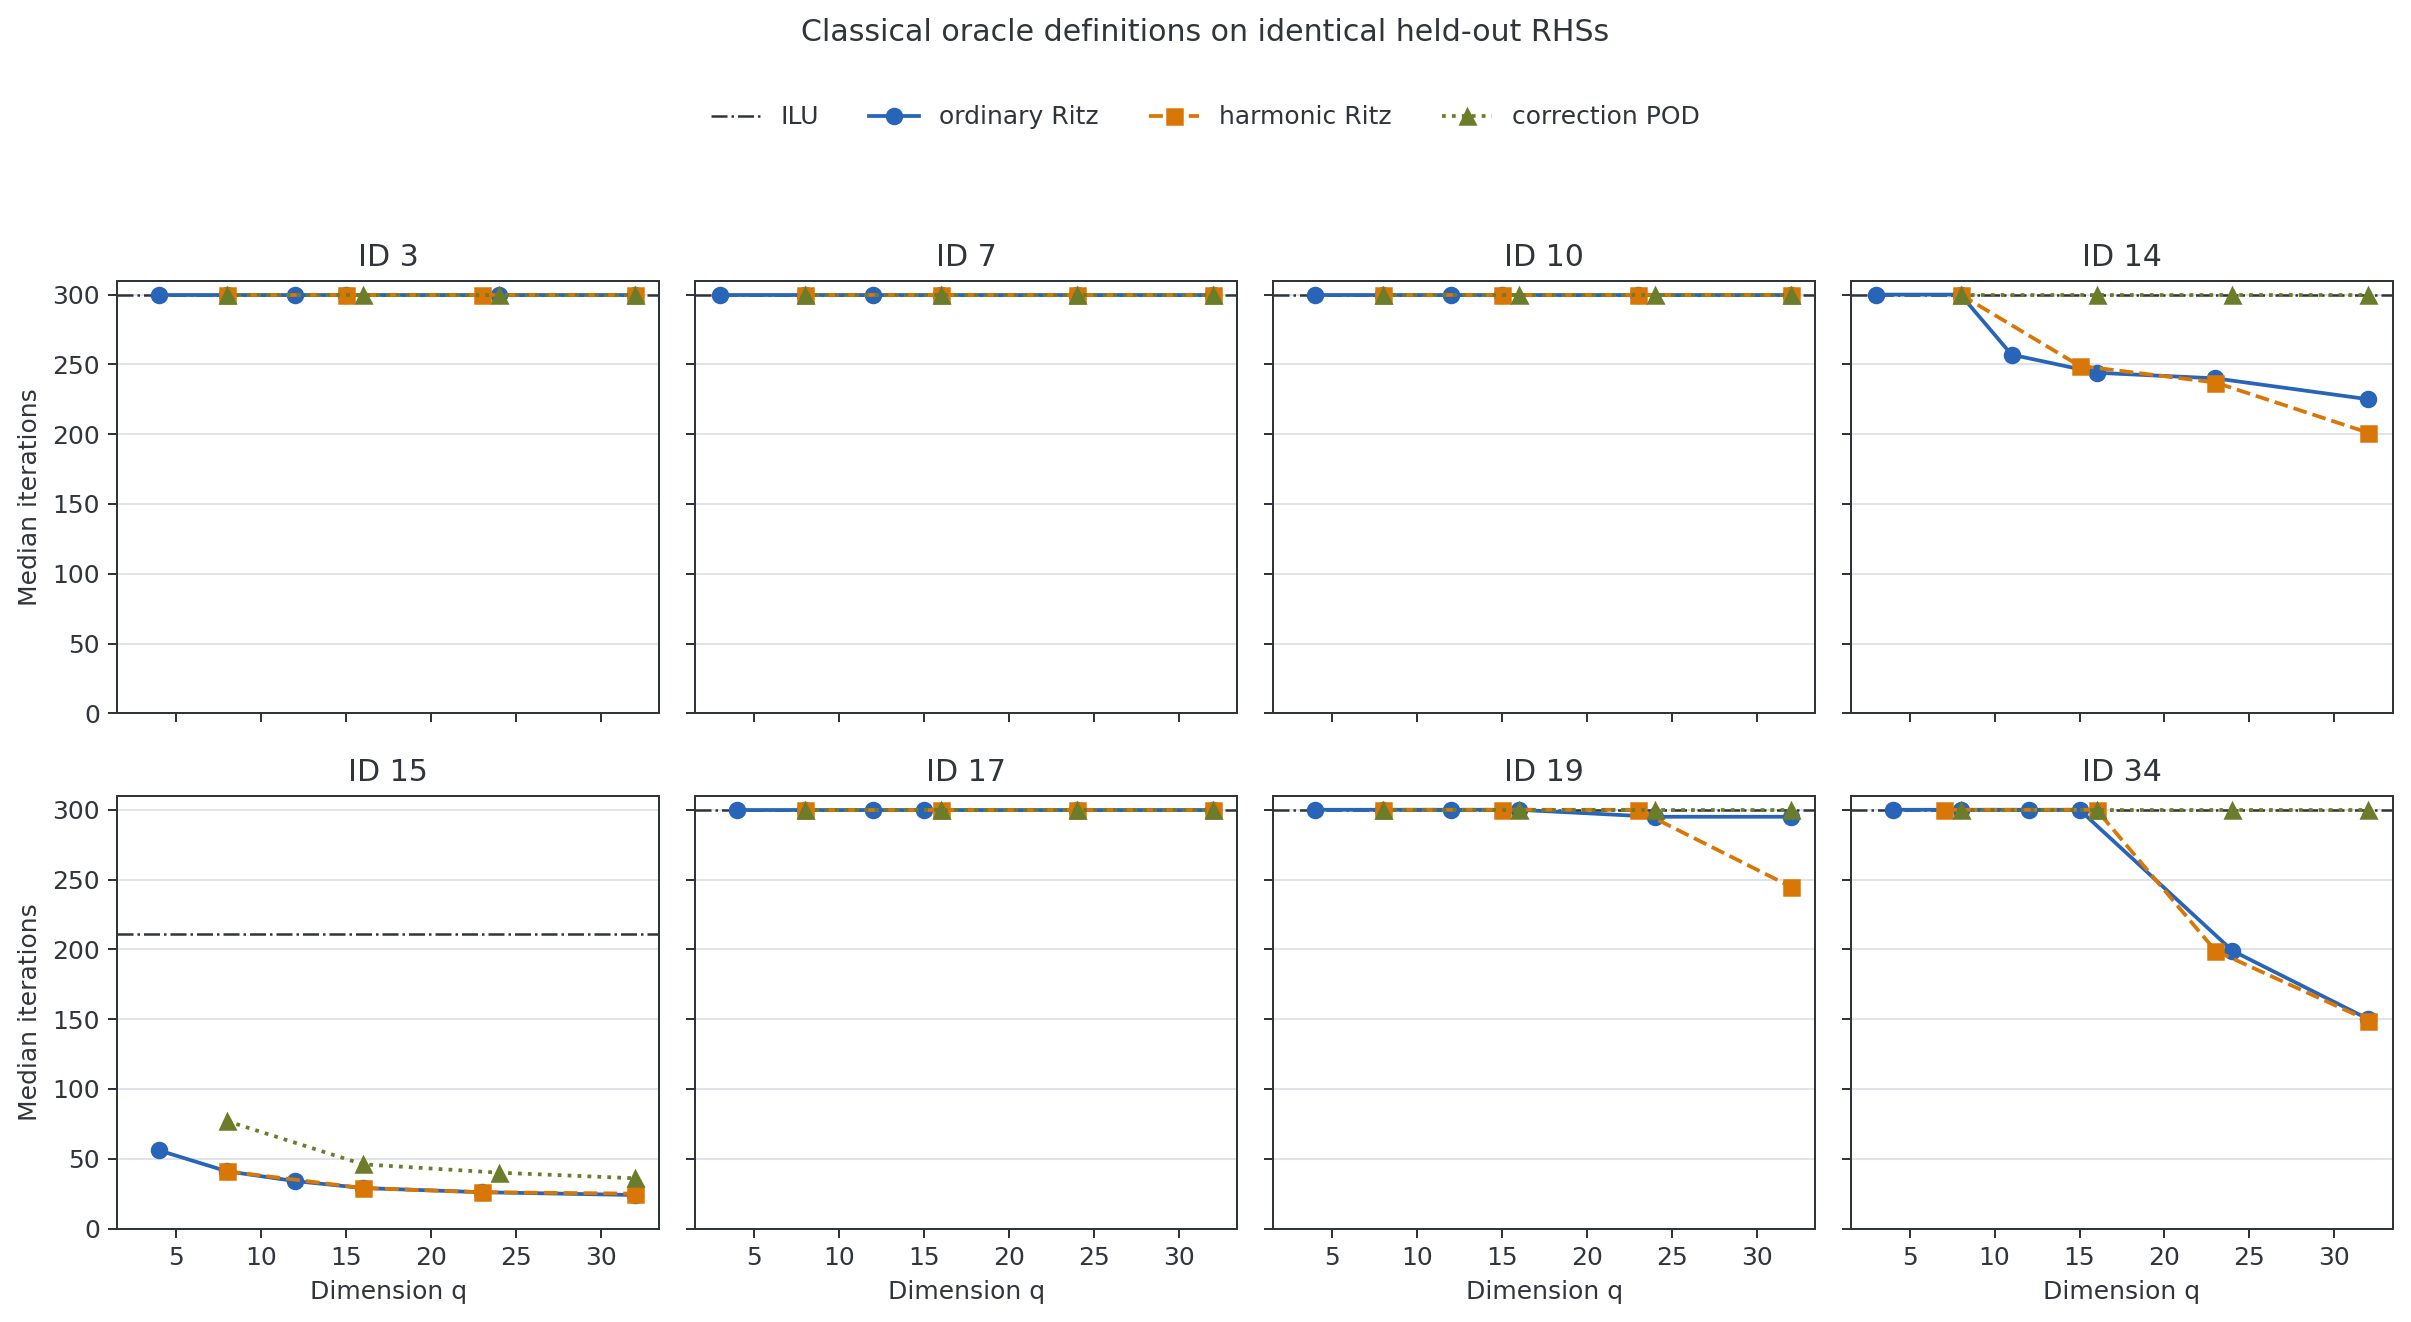
\includegraphics[width=0.90\textwidth]{figures/spatial_oracle_definitions.png}
\caption{Best ordinary Ritz, harmonic Ritz, and correction-POD outcomes through dimension 32.}
\label{fig:spatialdefs}
\end{figure}

The strongest contradiction concerned correction reconstruction and solver relevance. For IDs 17 and 34, correction POD had $q_{95}=q_{99}=1$. Held-out rank-eight projection errors were $1.76\times10^{-4}$ and 0.005, while both recycled solves reached the 300-step cap. A low-rank missing-action snapshot matrix does not guarantee an effective recycled-GMRES augmentation.

